% ══════════════════════════════════════════════════════════════════════════════════════════
%  Human cytokine dictionary: Immunology practical (slides, v3)
%  Build:  python slides/v3/make_figures.py   (figures, numbers and tables from the notebook)
%          cd slides/v3 && latexmk -xelatex main.tex
% ══════════════════════════════════════════════════════════════════════════════════════════
\documentclass[aspectratio=169,10pt]{beamer}
\usetheme[progressbar=frametitle,numbering=fraction,sectionpage=progressbar]{metropolis}

\usepackage{iftex}
\ifPDFTeX\usepackage[T1]{fontenc}\usepackage[utf8]{inputenc}\fi
\usepackage{amsmath,amssymb}
\usepackage{booktabs}
\usepackage{array}
\usepackage{graphicx}
\usepackage{xcolor}
\usepackage{listings}
\usepackage{url}
\usepackage{tikz}
\usetikzlibrary{arrows.meta,positioning,calc,fit,backgrounds,shapes.geometric,decorations.pathreplacing,matrix}
\usepackage{appendixnumberbeamer}
\graphicspath{{img/}}

\ifXeTeX
  \setsansfont[Extension=.otf,UprightFont=*-Regular,BoldFont=*-Bold,ItalicFont=*-Italic,BoldItalicFont=*-BoldItalic]{FiraSans}
  \setmonofont[Extension=.otf,UprightFont=*-Regular,BoldFont=*-Bold,Scale=0.92]{FiraMono}
\fi
\newcommand{\numnsamples}{4\,224}
\newcommand{\numngenesraw}{18\,120}
\newcommand{\numngenes}{15\,535}
\newcommand{\numngenesremoved}{2\,585}
\newcommand{\numumiMono}{6\,747}
\newcommand{\numumiNK}{3\,147}
\newcommand{\numpbsratio}{5.3}
\newcommand{\numtoptwentycpm}{35\%}
\newcommand{\numtoptwentylog}{1.6\%}
\newcommand{\numpcaone}{66}
\newcommand{\numpcatwo}{17}
\newcommand{\numpcathree}{3.4}
\newcommand{\numpcafirstfour}{88}
\newcommand{\numntested}{12\,743}
\newcommand{\numnup}{1\,353}
\newcommand{\numndown}{1\,282}
\newcommand{\numnrawsig}{7\,239}
\newcommand{\numnadjsig}{6\,585}
\newcommand{\numnexpectedfp}{637}
\newcommand{\numnnullraw}{750}
\newcommand{\numnnulladj}{0}
\newcommand{\numtobs}{10.6}
\newcommand{\numpobs}{3.9\times10^{-7}}
\newcommand{\numlfcobs}{3.66}
\newcommand{\numfoldobs}{12.6}
\newcommand{\numkstar}{6\,585}
\newcommand{\nummediancpm}{$-0.09$}
\newcommand{\nummediandeseq}{$+0.00$}
\newcommand{\numndegdeseq}{2\,635}
\newcommand{\numndegt}{2\,198}
\newcommand{\numndegboth}{1\,997}
\newcommand{\numreffect}{0.97}
                                    % numbers computed by make_figures.py

% ── colours (same hues as the notebook figures) ─────────────────────────────────────────
\definecolor{ucoblue}{HTML}{184F95}
\definecolor{bluemid}{HTML}{2A78D6}
\definecolor{accentred}{HTML}{E34948}
\definecolor{greyink}{HTML}{52514E}
\definecolor{softgrey}{HTML}{F0EFEC}
\definecolor{orangeslot}{HTML}{EB6834}
\definecolor{greenslot}{HTML}{1BAF7A}
\definecolor{yellowslot}{HTML}{EDA100}
\definecolor{magentaslot}{HTML}{E87BA4}
\setbeamercolor{frametitle}{bg=ucoblue,fg=white}
\setbeamercolor{progress bar}{fg=accentred,bg=ucoblue!30}
\setbeamercolor{alerted text}{fg=accentred}
\setbeamercolor{block title}{bg=ucoblue!85,fg=white}
\setbeamercolor{block body}{bg=softgrey,fg=black}
\setbeamercolor{title separator}{fg=accentred}
\setbeamercolor{section title}{fg=ucoblue}
\setbeamerfont{block title}{size=\small}
\setbeamertemplate{navigation symbols}{}

% ── helpers ───────────────────────────────────────────────────────────────────────────
\newcommand{\gene}[1]{\textit{#1}}
\newcommand{\code}[1]{\texttt{#1}}
\newcommand{\IFNg}{IFN-$\gamma$}
\newcommand{\figfit}[2][0.66]{\includegraphics[width=\linewidth,height=#1\textheight,keepaspectratio]{#2}}
\newcommand{\lfc}{\log_2\mathrm{FC}}
\newcommand{\timebox}[1]{\hfill{\footnotesize\textcolor{greyink}{$\circ$ #1}}}

\lstset{basicstyle=\ttfamily\scriptsize,keywordstyle=\color{bluemid}\bfseries,commentstyle=\color{greyink}\itshape,
        stringstyle=\color{accentred},showstringspaces=false,frame=single,rulecolor=\color{ucoblue!40},
        backgroundcolor=\color{softgrey},language=Python,columns=fullflexible,keepspaces=true,
        literate={→}{{$\rightarrow$}}1}

\title{Human cytokine dictionary}
\subtitle{From raw counts to differential expression\\ AnnData $\cdot$ normalization $\cdot$ PCA $\cdot$ differential analysis}
\author{Martin Garrido-Rodriguez}
\institute{UCO $\cdot$ Immunology practical}
\date{Based on Oesinghaus \emph{et al.} (2025), \emph{A single-cell cytokine dictionary of human peripheral blood}}

\begin{document}

\maketitle

% ════════════════════════════════════════════════════════════════════════════════════════
\begin{frame}{Plan of the practical: 2 h 30 min}
  \centering
  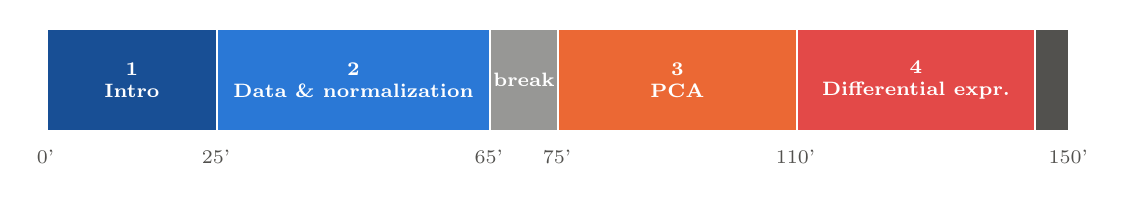
\begin{tikzpicture}[font=\scriptsize, every node/.style={align=center},
      seg/.style={draw=white,thick,minimum height=1.3cm,text=white,font=\scriptsize\bfseries,inner sep=1pt}]
    \def\u{0.0866}   % cm per minute, total width = 150 min = 13 cm
    \node[seg,fill=ucoblue,       minimum width={25*\u cm}, anchor=west] at (0,0)   {1\\ Intro};
    \node[seg,fill=bluemid,       minimum width={40*\u cm}, anchor=west] at (25*\u,0)  {2\\ Data \& normalization};
    \node[seg,fill=greyink!60,    minimum width={10*\u cm}, anchor=west] at (65*\u,0)  {break};
    \node[seg,fill=orangeslot,    minimum width={35*\u cm}, anchor=west] at (75*\u,0)  {3\\ PCA};
    \node[seg,fill=accentred,     minimum width={35*\u cm}, anchor=west] at (110*\u,0) {4\\ Differential expr.};
    \node[seg,fill=greyink,       minimum width={5*\u cm},  anchor=west] at (145*\u,0) {};
    \foreach \t/\x in {0/0,25/25,65/65,75/75,110/110,150/150}
      \node[below=0.12cm,text=greyink] at (\x*\u,-0.65) {\t'};
  \end{tikzpicture}

  \vspace{0.45cm}
  \small
  \begin{tabular}{@{}p{0.07\linewidth}p{0.47\linewidth}p{0.18\linewidth}p{0.17\linewidth}@{}}
    \toprule
    \textbf{Part} & \textbf{Topic} & \textbf{Format} & \textbf{Time}\\\midrule
    \textbf{1} & Introduction: Python, Jupyter, Colab, RNA-seq, single-cell, pseudobulk, dataset, AnnData & slides & 25 min\\[2pt]
    \textbf{2} & Manipulating and normalizing the data & notebook & 40 min\\[2pt]
    & \textit{Break} & & 10 min\\[2pt]
    \textbf{3} & Principal Component Analysis: one analysis to rule them all & slides + notebook & 35 min\\[2pt]
    \textbf{4} & Differential expression: cytokine vs control & slides + notebook & 35 min\\[2pt]
    & Wrap-up & & 5 min\\
    \bottomrule
  \end{tabular}
\end{frame}

% ════════════════════════════════════════════════════════════════════════════════════════
\section{Part 1: Introduction}

\begin{frame}[fragile]{What is Python?}
  \begin{columns}[T]
    \begin{column}{0.52\linewidth}
      \begin{itemize}\setlength\itemsep{4pt}
        \item A \alert{general-purpose programming language}: free, readable, with a huge community.
        \item You describe \emph{what to do} step by step, and the computer does it, on 10 or on 10 million samples.
        \item In science it is the \alert{glue} between data and analysis. Packages we use today:
      \end{itemize}
      \small
      \begin{tabular}{@{}ll@{}}
        \code{numpy} & arrays and linear algebra\\
        \code{pandas} & tables\\
        \code{scipy}, \code{statsmodels} & statistics\\
        \code{matplotlib} & plots\\
        \code{scikit-learn} & machine learning\\
        \code{anndata} & omics data containers\\
      \end{tabular}
    \end{column}
    \begin{column}{0.46\linewidth}
\begin{lstlisting}
genes  = ["STAT1", "CXCL9", "ACTB"]
counts = {"STAT1": 73853, "ACTB": 36500}
total  = sum(counts.values())
print(f"{total:,} UMIs in total")
\end{lstlisting}
      \vspace{0.15cm}
      \begin{block}{You do not need to be a programmer today}
        We provide the code. Your job: \textbf{run it, read the output, understand what the numbers mean}.
      \end{block}
    \end{column}
  \end{columns}
\end{frame}

\begin{frame}{What is a Jupyter notebook?}
  \begin{columns}[c]
    \begin{column}{0.56\linewidth}
      \centering
      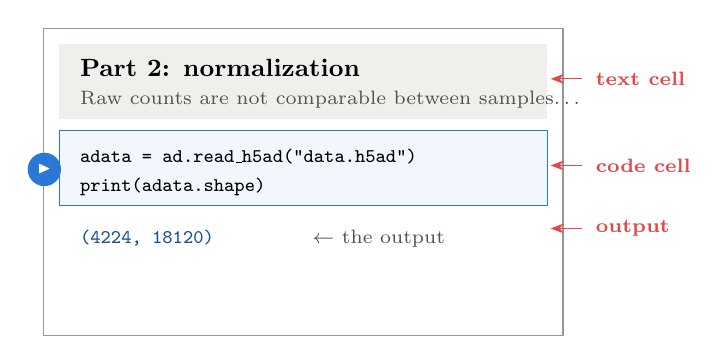
\begin{tikzpicture}[font=\scriptsize, every node/.style={align=left}]
        \node[draw=greyink!60,fill=white,minimum width=6.6cm,minimum height=3.9cm,anchor=north west] (page) at (0,0) {};
        % markdown cell
        \node[draw=none,fill=softgrey,minimum width=6.2cm,minimum height=0.95cm,anchor=north west] (md) at (0.2,-0.2) {};
        \node[anchor=north west,font=\small\bfseries] at (0.35,-0.28) {Part 2: normalization};
        \node[anchor=north west,font=\scriptsize,text=greyink] at (0.35,-0.68) {Raw counts are not comparable between samples\ldots};
        % code cell
        \node[draw=bluemid,fill=bluemid!6,minimum width=6.2cm,minimum height=0.95cm,anchor=north west] (code) at (0.2,-1.3) {};
        \node[anchor=north west,font=\ttfamily\scriptsize] at (0.35,-1.42) {adata = ad.read\_h5ad("data.h5ad")};
        \node[anchor=north west,font=\ttfamily\scriptsize] at (0.35,-1.78) {print(adata.shape)};
        \node[circle,fill=bluemid,text=white,inner sep=2pt,font=\tiny\bfseries] at (0.02,-1.8) {$\blacktriangleright$};
        % output
        \node[anchor=north west,font=\ttfamily\scriptsize,text=ucoblue] at (0.35,-2.45) {(4224, 18120)};
        \node[anchor=north west,font=\scriptsize,text=greyink] at (3.3,-2.45) {$\leftarrow$ the output};
        % labels
        \node[anchor=west,text=accentred,font=\scriptsize\bfseries] at (6.9,-0.65) {text cell};
        \node[anchor=west,text=accentred,font=\scriptsize\bfseries] at (6.9,-1.75) {code cell};
        \node[anchor=west,text=accentred,font=\scriptsize\bfseries] at (6.9,-2.55) {output};
        \draw[accentred,-{Stealth}] (6.85,-0.65) -- (6.45,-0.65);
        \draw[accentred,-{Stealth}] (6.85,-1.75) -- (6.45,-1.75);
        \draw[accentred,-{Stealth}] (6.85,-2.55) -- (6.45,-2.55);
      \end{tikzpicture}
    \end{column}
    \begin{column}{0.42\linewidth}\small
      \begin{itemize}\setlength\itemsep{3pt}
        \item A document that mixes \alert{text, code and results}.
        \item Two kinds of cells: \textbf{text} (Markdown) and \textbf{code} (Python).
        \item Run a cell: \alert{Shift\,+\,Enter}. The output appears below it.
        \item A \textbf{kernel} (the Python process behind the notebook) \alert{remembers} variables: run the cells \textbf{in order}.
        \item Restart the kernel $\Rightarrow$ memory is wiped.
      \end{itemize}
    \end{column}
  \end{columns}
\end{frame}

\begin{frame}{How are we going to run it? Google Colab}
  \begin{columns}[c]
    \begin{column}{0.60\linewidth}
      \centering
      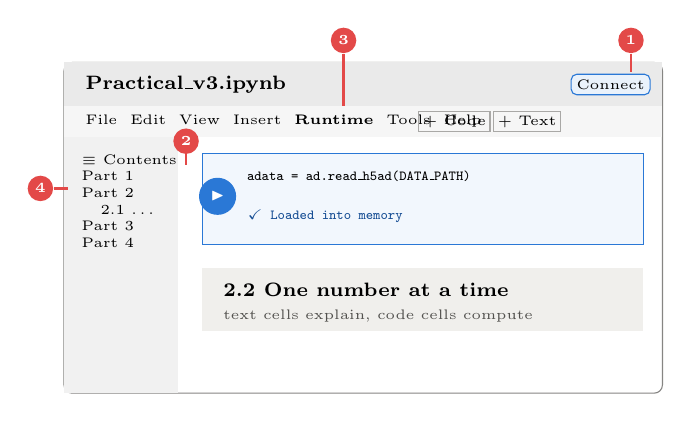
\begin{tikzpicture}[font=\scriptsize, every node/.style={align=left}]
        \draw[rounded corners=3pt,draw=greyink!70,fill=white] (0,0) rectangle (7.6,-4.2);
        \fill[greyink!12] (0,0) rectangle (7.6,-0.55);
        \node[anchor=west,font=\scriptsize\bfseries] at (0.15,-0.28) {Practical\_v3.ipynb};
        \node[anchor=east,draw=bluemid,fill=bluemid!10,rounded corners=2pt,inner sep=2pt,font=\tiny] at (7.45,-0.28) {Connect};
        \fill[greyink!5] (0,-0.55) rectangle (7.6,-0.95);
        \node[anchor=west,font=\tiny] at (0.15,-0.75) {File\ \ Edit\ \ View\ \ Insert\ \ \textbf{Runtime}\ \ Tools\ \ Help};
        \node[anchor=west,font=\tiny,draw=greyink!50,inner sep=1.5pt] at (4.5,-0.75) {+ Code};
        \node[anchor=west,font=\tiny,draw=greyink!50,inner sep=1.5pt] at (5.45,-0.75) {+ Text};
        \fill[greyink!8] (0,-0.95) rectangle (1.45,-4.2);
        \node[anchor=north west,font=\tiny] at (0.1,-1.05) {$\equiv$ Contents\\ Part 1\\ Part 2\\ \quad 2.1 \ldots\\ Part 3\\ Part 4};
        \node[draw=bluemid,fill=bluemid!6,minimum width=5.6cm,minimum height=1.15cm,anchor=north west] at (1.75,-1.15) {};
        \node[anchor=north west,font=\ttfamily\tiny] at (2.2,-1.25) {adata = ad.read\_h5ad(DATA\_PATH)};
        \node[circle,fill=bluemid,text=white,inner sep=2.5pt,font=\tiny] at (1.95,-1.7) {$\blacktriangleright$};
        \node[anchor=north west,font=\ttfamily\tiny,text=ucoblue] at (2.2,-1.75) {\checkmark\ Loaded into memory};
        \node[draw=none,fill=softgrey,minimum width=5.6cm,minimum height=0.8cm,anchor=north west] at (1.75,-2.6) {};
        \node[anchor=north west,font=\scriptsize\bfseries] at (1.9,-2.68) {2.2 One number at a time};
        \node[anchor=north west,font=\tiny,text=greyink] at (1.9,-3.02) {text cells explain, code cells compute};
        % numbered callouts
        \foreach \n/\x/\y/\tx/\ty in {1/7.2/0.28/7.2/-0.12, 2/1.55/-1.0/1.55/-1.3, 3/3.55/0.28/3.55/-0.55, 4/-0.3/-1.6/0.05/-1.6} {
          \node[circle,fill=accentred,text=white,inner sep=1.5pt,font=\tiny\bfseries] (c\n) at (\x,\y) {\n};
          \draw[accentred,thick] (c\n) -- (\tx,\ty);
        }
      \end{tikzpicture}
    \end{column}
    \begin{column}{0.38\linewidth}\small
      \begin{itemize}\setlength\itemsep{3pt}
        \item Jupyter in your \alert{browser}: nothing to install. Free, with a Google account.
        \item Your code runs on a \alert{temporary computer} in Google's cloud.
      \end{itemize}
      \vspace{0.1cm}
      \begin{enumerate}\setlength\itemsep{2pt}\footnotesize
        \item[\textcolor{accentred}{\textbf{1}}] \textbf{Connect} to a session
        \item[\textcolor{accentred}{\textbf{2}}] $\blacktriangleright$ \textbf{run} a cell
        \item[\textcolor{accentred}{\textbf{3}}] \textbf{Runtime} menu: run all, restart
        \item[\textcolor{accentred}{\textbf{4}}] \textbf{Table of contents}: jump between parts
      \end{enumerate}
    \end{column}
  \end{columns}
\end{frame}

\begin{frame}{Colab survival kit}
  \begin{columns}[T]
    \begin{column}{0.52\linewidth}
      \small
      \begin{tabular}{@{}>{\ttfamily}p{0.38\linewidth}p{0.58\linewidth}@{}}
        \toprule
        \textrm{\textbf{Shortcut}} & \textbf{What it does}\\\midrule
        Shift+Enter & run the cell and go to the next\\
        Ctrl+Enter & run the cell and stay\\
        Ctrl+M B & insert a cell below\\
        Ctrl+M D & delete the cell\\
        \bottomrule
      \end{tabular}
      \vspace{0.3cm}

      \textbf{If something breaks}
      \begin{itemize}\footnotesize\setlength\itemsep{2pt}
        \item \textbf{Runtime $\rightarrow$ Restart session}, then run from the top.
        \item Fell behind in Part 2? Use the \alert{catch-up cell} at the start of Part 3.
      \end{itemize}
    \end{column}
    \begin{column}{0.44\linewidth}
      \begin{block}{Good to know}
        \footnotesize
        \begin{itemize}\setlength\itemsep{3pt}
          \item Sessions are \alert{temporary}: files and variables disappear when it ends. We download the data at the start (about a minute).
          \item An idle session disconnects: reconnect and re-run.
          \item Cells whose title ends with \emph{``run once, no need to read''} are collapsed on purpose: helper code for the plots.
          \item To keep your changes: \textbf{File $\rightarrow$ Save a copy in Drive}.
        \end{itemize}
      \end{block}
    \end{column}
  \end{columns}
\end{frame}

% ────────────────────────────────────────────────────────────────────────────────────────
\begin{frame}{What is transcriptomics via RNA-seq?}
  \centering
  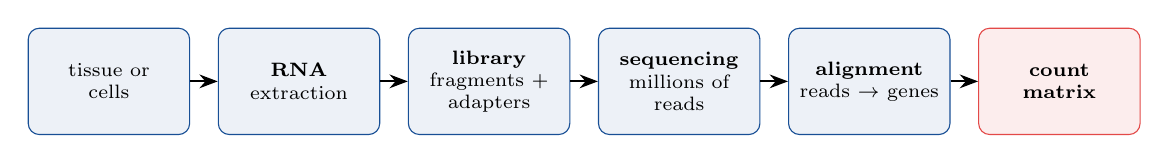
\begin{tikzpicture}[font=\scriptsize, every node/.style={align=center},
      stp/.style={draw=ucoblue,fill=ucoblue!8,rounded corners,minimum height=1.35cm,minimum width=2.05cm,inner sep=2pt}]
    \node[stp] (a) {tissue or\\ cells};
    \node[stp,right=0.35cm of a] (b) {\textbf{RNA}\\ extraction};
    \node[stp,right=0.35cm of b] (c) {\textbf{library}\\ fragments +\\ adapters};
    \node[stp,right=0.35cm of c] (d) {\textbf{sequencing}\\ millions of\\ reads};
    \node[stp,right=0.35cm of d] (e) {\textbf{alignment}\\ reads $\to$ genes};
    \node[stp,right=0.35cm of e,fill=accentred!10,draw=accentred] (f) {\textbf{count}\\ \textbf{matrix}};
    \foreach \x/\y in {a/b,b/c,c/d,d/e,e/f} \draw[-{Stealth},thick] (\x) -- (\y);
  \end{tikzpicture}
  \vspace{0.35cm}

  \begin{columns}[T]
    \begin{column}{0.5\linewidth}\small
      \begin{itemize}\setlength\itemsep{3pt}
        \item The \alert{transcriptome} is the set of all RNA molecules in a sample: which genes are \emph{on}, and how much.
        \item \textbf{Bulk RNA-seq} measures \alert{one average profile per sample}: all cells are mixed.
        \item A \textbf{count} is the number of molecules (or reads) assigned to a gene.
      \end{itemize}
    \end{column}
    \begin{column}{0.46\linewidth}
      \centering\footnotesize
      \begin{tabular}{lrrr}
        \toprule
        gene & sample 1 & sample 2 & sample 3\\\midrule
        \gene{STAT1} & 5\,310 & 12\,874 & 4\,990\\
        \gene{CXCL9} & 12 & 1\,950 & 9\\
        \gene{ACTB} & 36\,500 & 41\,200 & 33\,800\\
        $\vdots$ & $\vdots$ & $\vdots$ & $\vdots$\\
        \bottomrule
      \end{tabular}\\[2pt]
      \scriptsize a count matrix: \alert{genes $\times$ samples} (illustrative numbers)
    \end{column}
  \end{columns}
\end{frame}

\begin{frame}{Bulk and single-cell RNA-seq: the two workflows}
  \begin{columns}[c]
    \begin{column}{0.3\linewidth}
      \centering\includegraphics[width=\linewidth,height=0.8\textheight,keepaspectratio]{tzec_fig1_bulk.png}
    \end{column}
    \begin{column}{0.3\linewidth}
      \centering\includegraphics[width=\linewidth,height=0.8\textheight,keepaspectratio]{tzec_fig2_sc.png}
    \end{column}
    \begin{column}{0.36\linewidth}\small
      \begin{itemize}\setlength\itemsep{4pt}
        \item Same logic, different unit: a \alert{sample} (bulk) or a \alert{cell} (single-cell).
        \item Both end in a \alert{count matrix}, which is then normalized and analysed (differential expression, enrichment\ldots).
        \item Single-cell adds \alert{barcoding} to trace each read to its cell, and quality control per cell.
      \end{itemize}
      {\tiny Figures 1 and 2 of Tzec-Interi\'an \emph{et al.}\ 2025, \emph{Quant.\ Biol.}\ (CC BY)}
    \end{column}
  \end{columns}
\end{frame}

\begin{frame}{Single-cell transcriptomics: one profile per cell}
  \begin{columns}[c]
    \begin{column}{0.5\linewidth}
      \centering
      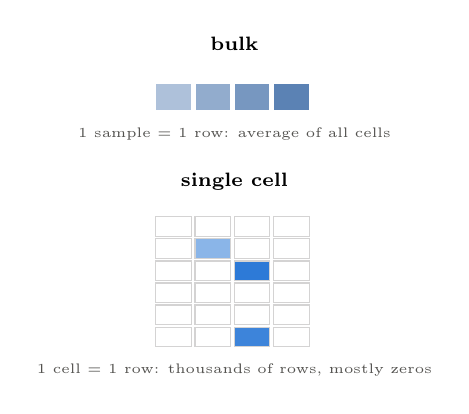
\begin{tikzpicture}[font=\scriptsize, every node/.style={align=center}]
        % bulk
        \node[font=\scriptsize\bfseries] at (1.0,2.6) {bulk};
        \foreach \c in {0,...,3} { \fill[ucoblue!\the\numexpr 35+\c*12\relax,draw=white] (\c*0.5,2.1) rectangle ++(0.45,-0.35); }
        \node[font=\tiny,text=greyink] at (1.0,1.45) {1 sample = 1 row: average of all cells};
        % single cell
        \node[font=\scriptsize\bfseries] at (1.0,0.85) {single cell};
        \foreach \r in {0,...,5} {
          \foreach \c in {0,...,3} {
            \pgfmathsetmacro{\v}{ifthenelse(rnd>0.72,rnd*65+35,0)}
            \fill[bluemid!\v!white,draw=greyink!25] (\c*0.5,0.4-\r*0.28) rectangle ++(0.45,-0.25);
          }
        }
        \node[font=\tiny,text=greyink] at (1.0,-1.55) {1 cell = 1 row: thousands of rows, mostly zeros};
      \end{tikzpicture}
    \end{column}
    \begin{column}{0.48\linewidth}\small
      \begin{tabular}{@{}>{\raggedright\arraybackslash}p{0.2\linewidth}>{\raggedright\arraybackslash}p{0.25\linewidth}>{\raggedright\arraybackslash}p{0.45\linewidth}@{}}
        \toprule
        & \textbf{bulk} & \textbf{single-cell}\\\midrule
        unit & sample & cell\\
        rows & tens & $10^4$--$10^7$\\
        zeros & few & most entries\\
        reveals & average & cell types and rare cells\\
        \bottomrule
      \end{tabular}
      \vspace{0.25cm}
      \begin{itemize}\footnotesize\setlength\itemsep{3pt}
        \item Every cell gets a \alert{barcode}, so reads can be traced back to their cell.
        \item Cell types are then identified by clustering and \emph{marker genes} (e.g.\ \gene{LYZ} for monocytes, \gene{CD3E} for T cells).
      \end{itemize}
    \end{column}
  \end{columns}
\end{frame}

\begin{frame}{Single-cell by combinatorial indexing (split-pool barcoding)}
  \centering
  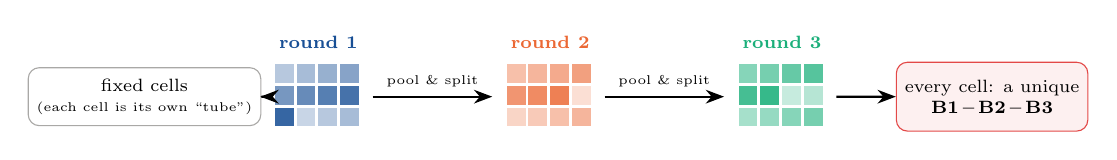
\begin{tikzpicture}[scale=0.92,transform shape,font=\scriptsize, every node/.style={align=center}]
    % plates: 3 small grids
    \foreach \p/\x/\col in {1/0.3/ucoblue, 2/3.5/orangeslot, 3/6.7/greenslot} {
      \foreach \r in {0,...,2} \foreach \c in {0,...,3} {
        \pgfmathsetmacro{\sh}{20+mod((\r*4+\c)*7+\p*11,70)}
        \fill[\col!\sh!white] (\x+\c*0.3,-\r*0.3) rectangle ++(0.26,-0.26);
      }
      \node[font=\scriptsize\bfseries,text=\col] at (\x+0.6,0.3) {round \p};
    }
    \node[draw=greyink!50,rounded corners,minimum width=1.9cm,minimum height=0.8cm,font=\scriptsize] (cells) at (-1.5,-0.45) {fixed cells\\ \tiny (each cell is its own ``tube'')};
    \draw[-{Stealth},thick] (cells) -- (0.1,-0.45);
    \draw[-{Stealth},thick] (1.65,-0.45) -- node[above,font=\tiny] {pool \& split} (3.3,-0.45);
    \draw[-{Stealth},thick] (4.85,-0.45) -- node[above,font=\tiny] {pool \& split} (6.5,-0.45);
    \node[draw=accentred,fill=accentred!8,rounded corners,minimum width=2.5cm,minimum height=0.95cm] (res) at (10.2,-0.45) {every cell: a unique\\ \textbf{B1\,--\,B2\,--\,B3}};
    \draw[-{Stealth},thick] (8.05,-0.45) -- (res);
  \end{tikzpicture}
  \vspace{0.3cm}

  \begin{columns}[T]
    \begin{column}{0.54\linewidth}\small
      \begin{itemize}\setlength\itemsep{3pt}
        \item In each round the cells are \alert{distributed in wells at random}; every well adds its own barcode to the RNA of the cells inside it.
        \item After three rounds the chance that two cells share the same three barcodes is tiny: with 96 barcodes per round, $96^3\approx 880\,000$ combinations (illustrative).
        \item \textbf{No droplets, no cell isolation}: millions of cells in one experiment.
      \end{itemize}
    \end{column}
    \begin{column}{0.42\linewidth}
      \begin{block}{In our data}
        \footnotesize
        The \alert{first-round barcode} is the well of the stimulation plate, i.e.\ the \alert{condition}: donor $\times$ cytokine. It is the \code{bc1\_well} column of the raw file.\\[2pt]
        The PBS control was spread over \alert{6 wells}.
      \end{block}
    \end{column}
  \end{columns}
\end{frame}

\begin{frame}{Why do we need to pseudobulk first?}
  \centering
  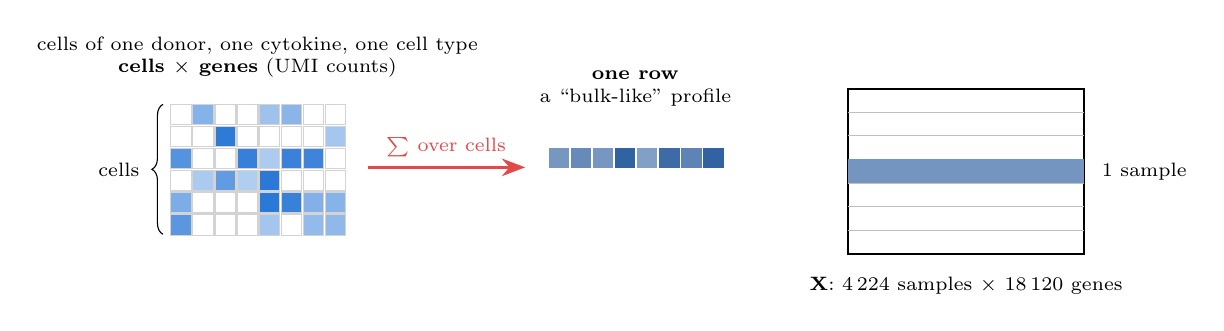
\begin{tikzpicture}[font=\scriptsize]
    \foreach \r in {0,...,5} {
      \foreach \c in {0,...,7} {
        \pgfmathsetmacro{\v}{ifthenelse(rnd>0.5,rnd*65+35,0)}
        \fill[bluemid!\v!white,draw=greyink!25] (\c*0.28,-\r*0.28) rectangle ++(0.26,-0.26);
      }
    }
    \node[align=center] at (1.1,0.6) {cells of one donor, one cytokine, one cell type\\ \textbf{cells $\times$ genes} (UMI counts)};
    \draw[decorate,decoration={brace,amplitude=4pt,mirror}] (-0.1,0) -- (-0.1,-1.65) node[midway,left=5pt] {cells};
    \draw[-{Stealth},very thick,accentred] (2.5,-0.8) -- node[above] {$\sum$ over cells} (4.5,-0.8);
    \foreach \c in {0,...,7} {
      \pgfmathsetmacro{\v}{rnd*45+50}
      \fill[ucoblue!\v] (4.8+\c*0.28,-0.55) rectangle ++(0.26,-0.26);
    }
    \node[align=center] at (5.9,0.2) {\textbf{one row}\\ a ``bulk-like'' profile};
    \draw[thick] (8.6,0.2) rectangle (11.6,-1.9);
    \foreach \r in {1,...,6} \draw[gray!50] (8.6,0.2-0.3*\r) -- (11.6,0.2-0.3*\r);
    \fill[ucoblue!60] (8.6,-0.7) rectangle (11.6,-1.0);
    \node[right] at (11.7,-0.85) {1 sample};
    \node at (10.1,-2.3) {\textbf{X}: \numnsamples\ samples $\times$ \numngenesraw\ genes};
  \end{tikzpicture}
  \vspace{0cm}

  \begin{itemize}\small\setlength\itemsep{2pt}
    \item \alert{The unit of replication is the donor, not the cell}: millions of cells come from only 12 people, and cells of one person are not independent. Testing cells as if they were replicates gives many false positives (\emph{pseudoreplication}).
    \item Single-cell counts are sparse and noisy; summed over thousands of cells they behave like \alert{bulk RNA-seq}, so standard, transparent statistics apply.
    \item It makes the data small: 9.7 million cells $\to$ \numnsamples\ samples.
  \end{itemize}
\end{frame}

% ────────────────────────────────────────────────────────────────────────────────────────
\begin{frame}{The dataset: the Human Cytokine Dictionary}
  \begin{columns}[c]
    \begin{column}{0.52\linewidth}
      \centering
      \includegraphics[width=\linewidth,height=0.74\textheight,keepaspectratio]{paper_fig1ab.png}\\[-1pt]
      {\tiny Oesinghaus \emph{et al.}\ 2025, Fig.\ 1a--b (CC BY-NC-ND 4.0)}
    \end{column}
    \begin{column}{0.44\linewidth}\small
      \begin{itemize}\setlength\itemsep{4pt}
        \item \alert{12 healthy donors} (6 female, 6 male; 34--75 years)
        \item \alert{90 cytokines} + a PBS control, in vitro for \alert{24 h}
        \item $\sim$\alert{9.7 million} PBMCs after quality control
        \item 16 cell types, annotated by marker genes (panel b)
      \end{itemize}
      \vspace{0.2cm}
      \footnotesize
      \textbf{Question of the paper:} what does every cytokine do to every immune cell type, and how much do people differ?
    \end{column}
  \end{columns}
\end{frame}

\begin{frame}{How the data were generated}
  \centering
  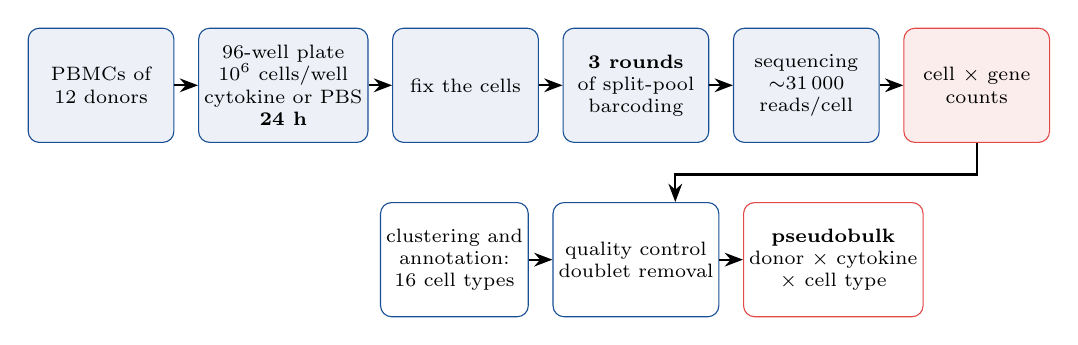
\begin{tikzpicture}[font=\scriptsize, every node/.style={align=center},
      stp/.style={draw=ucoblue,fill=ucoblue!8,rounded corners,minimum height=1.45cm,minimum width=1.85cm,inner sep=2pt},
      numdot/.style={circle,fill=accentred,text=white,inner sep=1.5pt,font=\tiny\bfseries}]
    \node[stp] (a) {PBMCs of\\ 12 donors};
    \node[stp,right=0.3cm of a] (b) {96-well plate\\ 10$^6$ cells/well\\ cytokine or PBS\\ \textbf{24 h}};
    \node[stp,right=0.3cm of b] (c) {fix the cells};
    \node[stp,right=0.3cm of c] (d) {\textbf{3 rounds}\\ of split-pool\\ barcoding};
    \node[stp,right=0.3cm of d] (e) {sequencing\\ $\sim$31\,000\\ reads/cell};
    \node[stp,right=0.3cm of e,fill=accentred!10,draw=accentred] (f) {cell $\times$ gene\\ counts};
    \foreach \x/\y in {a/b,b/c,c/d,d/e,e/f} \draw[-{Stealth},thick] (\x) -- (\y);
    \node[stp,below=0.75cm of d,fill=white] (g) {quality control\\ doublet removal};
    \node[stp,left=0.3cm of g,fill=white] (h) {clustering and\\ annotation:\\ 16 cell types};
    \node[stp,right=0.3cm of g,fill=white,draw=accentred] (i) {\textbf{pseudobulk}\\ donor $\times$ cytokine\\ $\times$ cell type};
    \draw[-{Stealth},thick] (f.south) |- ($(g.north)+(0.5,0.35)$) -- ($(g.north)+(0.5,0)$);
    \draw[-{Stealth},thick] (g) -- (i); \draw[-{Stealth},thick] (h) -- (g);
  \end{tikzpicture}
  \vspace{0.25cm}

  \footnotesize
  \begin{itemize}\setlength\itemsep{2pt}
    \item Barcoding with the Parse Biosciences GigaLab protocol; sublibraries of $\sim$100\,000 cells; sequencing on an Ultima UG-100.
    \item Cells kept with 400--7\,000 detected genes and $<15\,\%$ mitochondrial reads.
  \end{itemize}
\end{frame}

\begin{frame}{What is in the subset we work with?}
  \begin{columns}[T]
    \begin{column}{0.56\linewidth}
      \small
      \begin{tabular}{@{}>{\raggedright\arraybackslash}p{0.2\linewidth}>{\raggedright\arraybackslash}p{0.22\linewidth}>{\raggedright\arraybackslash}p{0.52\linewidth}@{}}
        \toprule
        & \textbf{paper} & \textbf{our practical}\\\midrule
        donors & 12 & 12\\[1pt]
        cytokines & 90 + PBS & 87 + PBS\\[1pt]
        cell types & 16 & 4: CD4 T, CD8 T, NK CD56\textsuperscript{low}, CD14 monocytes\\[1pt]
        unit & single cells & \alert{pseudobulk} samples\\[1pt]
        genes & all & \numngenesraw\ protein-coding ($\to$ \numngenes\ after filtering)\\
        \bottomrule
      \end{tabular}
    \end{column}
    \begin{column}{0.4\linewidth}
      \begin{block}{The design}
        \centering
        $4$ cell types\\ $\times$ $88$ conditions\\ \footnotesize(87 cytokines + PBS)\\ \normalsize $\times$ $12$ donors\\[3pt]
        $=$ \alert{\numnsamples\ samples}
      \end{block}
      \footnotesize
      The PBS control was measured in 6 wells; the file stores each well \emph{and} their total. We keep the total (bonus B1 of the notebook).
    \end{column}
  \end{columns}
\end{frame}

\begin{frame}{AnnData: a Python data structure for omics data}
  \begin{columns}[c]
    \begin{column}{0.38\linewidth}
      \centering
      \includegraphics[width=\linewidth,height=0.76\textheight,keepaspectratio]{anndata_schema.png}\\[-1pt]
      {\tiny AnnData schema (anndata documentation)}
    \end{column}
    \begin{column}{0.58\linewidth}\small
      \begin{itemize}\setlength\itemsep{3pt}
        \item \textbf{One object, several tables that always stay aligned.}
        \item \textcolor{ucoblue}{\textbf{\code{X}}}: the main matrix, $n_{\text{obs}}\times n_{\text{vars}}$
        \item \textcolor{yellowslot}{\textbf{\code{obs}}}: one row per \alert{observation} (sample or cell): metadata
        \item \textcolor{bluemid}{\textbf{\code{var}}}: one row per \alert{variable} (gene): metadata
        \item \textcolor{greenslot}{\textbf{\code{layers}}}: more matrices, same shape as \code{X}
        \item \code{obsm}, \code{varm}, \code{obsp}, \code{varp}, \code{uns}: embeddings (PCA), graphs, free-form results
      \end{itemize}
      \vspace{0.15cm}
      \begin{block}{Why it matters}
        \footnotesize Subsetting moves \emph{all} the tables together: no gene or sample can get out of sync with its metadata. Saved as an \code{.h5ad} file.
      \end{block}
    \end{column}
  \end{columns}
\end{frame}

\begin{frame}[fragile]{AnnData in our practical}
  \begin{columns}[T]
    \begin{column}{0.52\linewidth}
      \small
      \begin{tabular}{@{}>{\ttfamily}p{0.16\linewidth}>{\raggedright\arraybackslash}p{0.47\linewidth}>{\raggedright\arraybackslash}p{0.3\linewidth}@{}}
        \toprule
        \textrm{\textbf{slot}} & \textbf{our data} & \textbf{shape}\\\midrule
        X & raw counts, later $\log_2$(CPM+1) & \numnsamples\,$\times$\,\numngenesraw\\[2pt]
        obs & donor, cytokine, treatment, cell\_type, number of cells & \numnsamples\ rows\\[2pt]
        var & gene names, total counts & \numngenesraw\ rows\\[2pt]
        layers & \code{counts}, \code{cpm} & same as \code{X}\\[2pt]
        obsm & PCA scores (Part 3) & \numnsamples\,$\times$\,10\\
        \bottomrule
      \end{tabular}
    \end{column}
    \begin{column}{0.46\linewidth}
\begin{lstlisting}
# rows first (samples), then genes
adata[["Donor1|CD14_Mono|IFN-gamma"],
      ["STAT1"]]

mask = adata.obs["cell_type"] == "CD14_Mono"
adata[mask, ["IDO1", "CXCL10"]]
\end{lstlisting}
      \footnotesize The first selection is $1\times1$; the second one, $1\,056\times2$ (all monocyte samples).
    \end{column}
  \end{columns}
  \vspace{0.25cm}
  \begin{block}{Hands-on}
    \small Back to the notebook: \textbf{Part 1 setup} (install, load the data), then \textbf{Part 2}.
    \timebox{about 25 min for Part 1}
  \end{block}
\end{frame}

% ════════════════════════════════════════════════════════════════════════════════════════
\section{Part 2: Manipulating and normalizing the data}

\begin{frame}{Part 2 roadmap: 40 min, in the notebook}
  \small
  \begin{tabular}{@{}p{0.07\linewidth}p{0.6\linewidth}p{0.2\linewidth}@{}}
    \toprule
    \textbf{Step} & \textbf{Question} & \textbf{Time}\\\midrule
    \textbf{2.1} & Prepare the object & 3 min\\[3pt]
    \textbf{2.2} & What does the data look like? From \textbf{1 number} to the \textbf{whole matrix} & 10 min\\[3pt]
    \textbf{2.3} & What is a \textbf{count}? Why do libraries have different sizes? & 7 min\\[3pt]
    \textbf{2.4} & \textbf{Normalization}: what, why, how & 10 min\\[3pt]
    \textbf{2.5} & Why do we \textbf{filter} lowly expressed genes? & 5 min\\[3pt]
    \textbf{2.6} & \textbf{Heatmaps} before and after normalizing & 5 min\\
    \bottomrule
  \end{tabular}
  \vspace{0.3cm}

  \begin{block}{Goal}
    Understand what is inside the data and turn \alert{raw counts} into numbers we can \alert{compare} between samples and between genes.
  \end{block}
\end{frame}

\begin{frame}{2.2 From one number to the whole matrix}
  \centering
  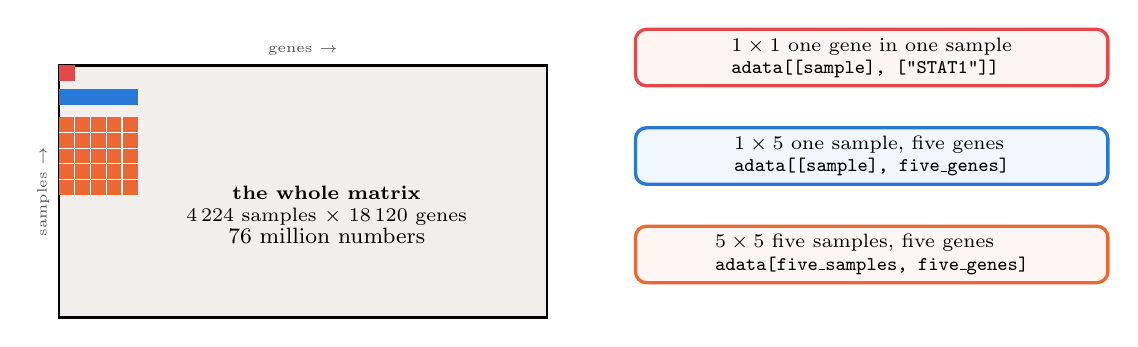
\begin{tikzpicture}[font=\scriptsize]
    % the big matrix
    \draw[thick,fill=softgrey] (0,0) rectangle (6.2,-3.2);
    \node[align=center] at (3.4,-1.9) {\textbf{the whole matrix}\\ \numnsamples\ samples $\times$ \numngenesraw\ genes\\ \footnotesize 76 million numbers};
    \node[above,font=\tiny,text=greyink] at (3.1,0) {genes $\rightarrow$};
    \node[rotate=90,above,font=\tiny,text=greyink] at (0,-1.6) {samples $\rightarrow$};
    % the three zoom levels, at the corner
    \fill[accentred] (0,0) rectangle ++(0.2,-0.2);
    \fill[bluemid]   (0,-0.3) rectangle ++(1.0,-0.2);
    \fill[orangeslot] (0,-0.65) rectangle ++(1.0,-1.0);
    \foreach \i in {1,...,4} { \draw[white] (\i*0.2,-0.65) -- (\i*0.2,-1.65); \draw[white] (0,-0.65-\i*0.2) -- (1.0,-0.65-\i*0.2); }
    % explanations
    \node[anchor=west,draw=accentred,very thick,rounded corners,fill=accentred!6,minimum width=6.0cm,align=left,inner sep=3pt] (a) at (7.3,0.1)
      {\textbf{$1\times1$} one gene in one sample\\ \ttfamily\scriptsize adata[[sample], ["STAT1"]]};
    \node[anchor=west,draw=bluemid,very thick,rounded corners,fill=bluemid!6,minimum width=6.0cm,align=left,inner sep=3pt] (b) at (7.3,-1.15)
      {\textbf{$1\times5$} one sample, five genes\\ \ttfamily\scriptsize adata[[sample], five\_genes]};
    \node[anchor=west,draw=orangeslot,very thick,rounded corners,fill=orangeslot!6,minimum width=6.0cm,align=left,inner sep=3pt] (c) at (7.3,-2.4)
      {\textbf{$5\times5$} five samples, five genes\\ \ttfamily\scriptsize adata[five\_samples, five\_genes]};
  \end{tikzpicture}

  \vspace{0.2cm}
  \begin{itemize}\small\setlength\itemsep{3pt}
    \item Every piece comes with its \alert{metadata}: \code{.obs} describes the samples (rows), \code{.var} the genes (columns).
    \item The 5\,$\times$\,5 table is just the top-left corner of the whole matrix: what we do next applies to \emph{all} of it.
  \end{itemize}
\end{frame}

\begin{frame}{2.3 What is a count?}
  \centering
  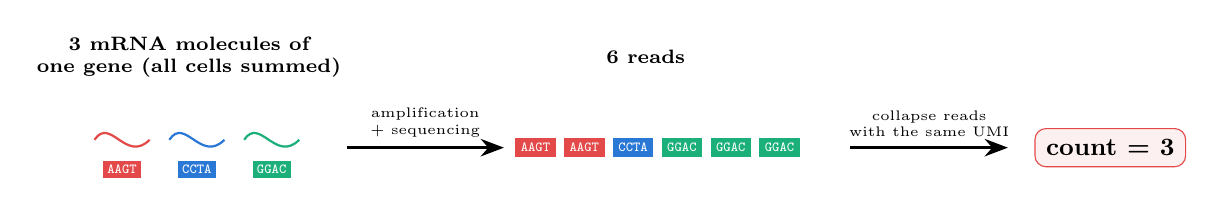
\begin{tikzpicture}[font=\scriptsize, every node/.style={align=center}]
    % molecules
    \node[font=\scriptsize\bfseries] at (1.2,1.15) {3 mRNA molecules of\\ one gene (all cells summed)};
    \foreach \i/\col/\u in {0/accentred/AAGT, 1/bluemid/CCTA, 2/greenslot/GGAC} {
      \draw[thick,\col] (\i*0.95,0.1) .. controls (\i*0.95+0.2,0.4) and (\i*0.95+0.4,-0.2) .. (\i*0.95+0.7,0.1);
      \node[fill=\col,text=white,inner sep=1.5pt,font=\tiny\ttfamily] at (\i*0.95+0.35,-0.28) {\u};
    }
    \draw[-{Stealth},very thick] (3.2,0) -- node[above,font=\tiny] {amplification\\ + sequencing} (5.2,0);
    % reads
    \node[font=\scriptsize\bfseries] at (7.0,1.15) {6 reads};
    \foreach \i/\col/\u in {0/accentred/AAGT, 1/accentred/AAGT, 2/bluemid/CCTA, 3/greenslot/GGAC, 4/greenslot/GGAC, 5/greenslot/GGAC} {
      \node[fill=\col,text=white,inner sep=2pt,font=\tiny\ttfamily] at (5.6+\i*0.62,0) {\u};
    }
    \draw[-{Stealth},very thick] (9.6,0) -- node[above,font=\tiny] {collapse reads\\ with the same UMI} (11.6,0);
    \node[draw=accentred,rounded corners,fill=accentred!8,inner sep=4pt,font=\small\bfseries] at (12.9,0) {count = 3};
  \end{tikzpicture}
  \vspace{0.3cm}

  \begin{columns}[T]
    \begin{column}{0.52\linewidth}\small
      \begin{itemize}\setlength\itemsep{3pt}
        \item A \textbf{UMI} (\emph{unique molecular identifier}) is a random tag added to each \emph{original} molecule.
        \item Counting \alert{distinct UMIs} instead of reads removes the PCR duplicates: one UMI $=$ one molecule.
      \end{itemize}
    \end{column}
    \begin{column}{0.44\linewidth}\small
      \begin{itemize}\setlength\itemsep{3pt}
        \item In a pseudobulk the count is \alert{summed over all the cells} of the sample.
        \item So a count is a non-negative integer that depends on the \textbf{biology} and on \textbf{how much material} we have.
      \end{itemize}
    \end{column}
  \end{columns}
\end{frame}

\begin{frame}{2.3 Library size: cells $\times$ UMIs per cell}
  \centering
  \figfit[0.5]{p2_libsize}\\[-1pt]
  \begin{columns}[c]
    \begin{column}{0.4\linewidth}
      \centering\scriptsize
      \begin{tabular}{lrrr}\toprule
 & cells & UMIs / cell & library size\\\midrule
CD4 T & 3\,041 & 2\,989 & 8.5\,M\\
CD8 T & 1\,302 & 3\,104 & 3.8\,M\\
NK & 407 & 3\,147 & 1.2\,M\\
Monocytes & 1\,238 & 6\,747 & 7.6\,M\\
\bottomrule\end{tabular}

    \end{column}
    \begin{column}{0.58\linewidth}\footnotesize
      \begin{itemize}\setlength\itemsep{2pt}
        \item \textbf{Library size} $L_i=\sum_j\text{count}_{ij}$: total counts of sample $i$.
        \item CD4 T cells are the most abundant, NK cells the rarest ($\sim$400 cells).
        \item Monocytes have \alert{\numumiMono\ UMIs per cell} vs $\sim$\numumiNK\ in lymphocytes: bigger cells, more mRNA.
        \item PBS controls are the sum of 6 wells: \alert{\numpbsratio$\times$ deeper}.
      \end{itemize}
    \end{column}
  \end{columns}
\end{frame}

\begin{frame}{2.4 Why normalize? An example}
  \begin{columns}[c]
    \begin{column}{0.56\linewidth}
      \figfit[0.62]{p2_toy}
    \end{column}
    \begin{column}{0.42\linewidth}\small
      \textit{Is ``cytokine'' used more in a 10-page article or in a 100-page review?} Compare \alert{frequencies}, not counts.
      \vspace{0.2cm}
      \begin{itemize}\setlength\itemsep{3pt}
        \item Same donor: a PBS control (deep) and an IFN-$\gamma$ sample (5$\times$ shallower). Gene B is an interferon-response gene.
        \item \alert{Raw counts}: every gene looks \emph{lower} with IFN-$\gamma$, even the induced interferon-response gene B.
        \item \alert{CPM}: A, C, D are unchanged and B is $4\times$ up. The right answer.
      \end{itemize}
    \end{column}
  \end{columns}
\end{frame}

\begin{frame}{CPM: counts per million}
  \[
    \text{CPM}_{ij}\;=\;\frac{\text{count}_{ij}}{L_i}\times 10^{6},\qquad L_i=\sum_{j}\text{count}_{ij}
  \]
  \centering
  \figfit[0.46]{p2_actb}\\[-2pt]
  \small \gene{ACTB}, a housekeeping gene, in monocytes (PBS samples included). After CPM it no longer follows the library size.
\end{frame}

\begin{frame}{The logarithm: across genes}
  \begin{columns}[c]
    \begin{column}{0.6\linewidth}
      \figfit[0.6]{p2_logvar}
    \end{column}
    \begin{column}{0.38\linewidth}\small
      \begin{itemize}\setlength\itemsep{3pt}
        \item In CPM, \alert{variance rises steeply with the mean}.
        \item The 20 most variable genes hold \numtoptwentycpm\ of the total variance in CPM\ldots{}
        \item \ldots{}and only \numtoptwentylog\ after $\log_2(\text{CPM}+1)$.
        \item PCA, clustering and $t$-tests are driven by variance: without the log, a few abundant genes decide everything.
      \end{itemize}
    \end{column}
  \end{columns}
\end{frame}

\begin{frame}{The logarithm and the pseudocount}
  \[ \text{log-CPM}_{ij}=\log_2\bigl(\text{CPM}_{ij}+1\bigr) \]
  \begin{columns}[T]
    \begin{column}{0.45\linewidth}
      \footnotesize\textbf{Fold changes become symmetric}\\[3pt]
      \scriptsize\setlength\tabcolsep{2.5pt}
      \begin{tabular}{@{}lccccccc@{}}
        \toprule
        fold change & $\times4$ & $\times2$ & $\times1.4$ & $\times1$ & $\times0.7$ & $\times0.5$ & $\times0.25$\\
        $\lfc$ & $+2$ & $+1$ & $+0.5$ & $0$ & $-0.5$ & $-1$ & $-2$\\
        \bottomrule
      \end{tabular}\\[4pt]
      The difference of two log-values \emph{is} the log fold change.
    \end{column}
    \begin{column}{0.53\linewidth}
      \footnotesize\textbf{Why ``+1''?}\\[3pt]
      \setlength\tabcolsep{2.5pt}
      \begin{tabular}{@{}lrrrr@{}}
        \toprule
        gene & ctrl & trt & $\lfc$ & $\lfc^{+1}$\\\midrule
        almost silent & 0.1 & 0.4 & $+2.00$ & $+0.35$\\
        silent $\to$ detected & 0 & 0.5 & $+\infty$ & $+0.58$\\
        moderate & 20 & 40 & $+1.00$ & $+0.97$\\
        high & 500 & 1000 & $+1.00$ & $+1.00$\\
        \bottomrule
      \end{tabular}\\[2pt]
      \scriptsize ctrl, trt = CPM; $\lfc^{+1}$ uses CPM\,$+1$.\\[3pt]
      The pseudocount shrinks fold changes of tiny numbers: ``I don't trust ratios of one or two molecules''.
    \end{column}
  \end{columns}
\end{frame}

\begin{frame}{2.5 Why filter lowly expressed genes?}
  \centering
  \figfit[0.38]{p2_poisson}\\[-2pt]
  \small The \alert{same gene measured twice} (no true change), at four expression levels (Poisson noise only)
  \begin{itemize}\small\setlength\itemsep{3pt}
    \item Low counts are \alert{pure sampling noise}: with 2 vs 4 molecules, a ``doubling'' is bad luck.
    \item They give \alert{false fold changes} and \alert{more tests} to correct for (Part 4).
  \end{itemize}
\end{frame}

\begin{frame}{The rule: $\geq$ 10 counts in $\geq$ 12 samples}
  \begin{columns}[c]
    \begin{column}{0.56\linewidth}
      \figfit[0.6]{p2_filter}
    \end{column}
    \begin{column}{0.42\linewidth}\small
      \begin{itemize}\setlength\itemsep{4pt}
        \item 12 = the number of donors: the size of one experimental group (the idea of \texttt{filterByExpr} in edgeR).
        \item A gene that never reaches 10 counts in a whole group cannot be tested anywhere.
        \item \alert{\numngenes\ of \numngenesraw\ genes} pass. The \numngenesremoved\ removed ones carry 0.011\,\% of all counts (e.g.\ olfactory receptors).
      \end{itemize}
    \end{column}
  \end{columns}
\end{frame}

\begin{frame}{2.6 Heatmaps: cell-type markers, before and after}
  \centering
  \figfit[0.72]{p2_heat_markers}
  \vspace{-0.15cm}\\
  \scriptsize
  \textbf{z-score per gene across samples:} $z_{gi}=(x_{gi}-\bar x_g)/s_g$ (red: above the gene's average). Columns: mean of the 12 donors. \alert{Before}: the PBS columns (deepest libraries) glow. \alert{After}: clean cell-type blocks.
\end{frame}

\begin{frame}{2.6 Heatmaps: genes of the immune response}
  \begin{columns}[c]
    \begin{column}{0.71\linewidth}
      \figfit[0.8]{p2_heat_immune}
    \end{column}
    \begin{column}{0.27\linewidth}\scriptsize
      Four cytokines, four pathways:
      \begin{itemize}\setlength\itemsep{3pt}
        \item \textbf{IFN-$\gamma$ / STAT1}: \gene{GBP1}, \gene{IDO1}, \gene{CXCL9}\ldots, strongest in monocytes
        \item \textbf{IL-4 / STAT6}: \gene{ALOX15}, \gene{CCL17}, \gene{FCER2}, monocytes
        \item \textbf{IL-1$\beta$ / NF-$\kappa$B}: \gene{IL6}, \gene{CXCL8}, \gene{CCL2}, monocytes
        \item \textbf{IL-2 / STAT5}: \gene{IL2RA}, \gene{GZMB}, \gene{CISH}, NK and T cells
      \end{itemize}
      \alert{Normalized: biology. Raw: sequencing depth.}\\[2pt]
      z-scores are for visualization only.
    \end{column}
  \end{columns}
\end{frame}

\begin{frame}{Your turn in the notebook (Part 2)}
  \small
  Cells that start with \code{\# CHANGE ME} contain parameters you can modify. Change them, re-run and see what happens:
  \vspace{0.2cm}

  \begin{tabular}{@{}>{\ttfamily}p{0.27\linewidth}>{\raggedright\arraybackslash}p{0.68\linewidth}@{}}
    \toprule
    \textrm{\textbf{Parameter}} & \textbf{Try\ldots}\\\midrule
    sample, genes5, samples5 & other samples and genes in the $1\times1$ and $5\times5$ tables: which marker is high in which cell type?\\[2pt]
    mask & another cell type and cytokines: is the raw count higher with the cytokine?\\[2pt]
    MIN\_COUNT, MIN\_SAMPLES & a stricter or looser gene filter: how many genes survive?\\[2pt]
    CELL\_TYPE\_MARKERS, IMMUNE\_GENES & your own genes in the before/after heatmaps\\
    \bottomrule
  \end{tabular}
\end{frame}

\begin{frame}{Part 2 in one slide}
  \footnotesize
  \begin{tabular}{@{}c>{\raggedright\arraybackslash}p{0.14\linewidth}>{\raggedright\arraybackslash}p{0.33\linewidth}>{\raggedright\arraybackslash}p{0.22\linewidth}>{\raggedright\arraybackslash}p{0.17\linewidth}@{}}
    \toprule
    & \textbf{Step} & \textbf{Fixes} & \textbf{Formula} & \textbf{Stored in}\\\midrule
    1 & CPM & different library sizes (between samples) & $\text{count}_{ij}/L_i\times10^6$ & \code{layers["cpm"]}\\[2pt]
    2 & $\log_2(\cdot+1)$ & dynamic range, mean--variance link (across genes) & $\log_2(\text{CPM}+1)$ & \code{adata.X}\\[2pt]
    3 & gene filter & noise and too many tests & $\geq10$ counts in $\geq12$ samples & rows of \code{adata}\\[2pt]
    4 & z-score per gene & gene baseline hides the pattern (heatmaps) & $(x_{gi}-\bar x_g)/s_g$ & not stored\\
    \bottomrule
  \end{tabular}
  \vspace{0.4cm}
  \begin{block}{Remember}
    \code{layers["counts"]} = raw counts \quad $\to$ \quad \code{layers["cpm"]} = CPM \quad $\to$ \quad \code{adata.X} = log$_2$(CPM+1)
  \end{block}
\end{frame}

\begin{frame}[standout]
  Break\\[6pt]
  {\Large 10 minutes}
\end{frame}

% ════════════════════════════════════════════════════════════════════════════════════════
\section{Part 3: Principal Component Analysis}

\begin{frame}{Part 3 roadmap: one analysis to rule them all (35 min)}
  \footnotesize
  \begin{columns}[T]
    \begin{column}{0.54\linewidth}
      \textbf{Slides} (10 min)
      \begin{itemize}\setlength\itemsep{1pt}
        \item Why dimensionality reduction?
        \item PCA as a \alert{rotation}
        \item \alert{SVD}: how it is computed
        \item \alert{Projection}: scores and loadings
        \item PCA across fields
      \end{itemize}
      \vspace{0.1cm}
      \textbf{Notebook} (25 min)
      \begin{itemize}\setlength\itemsep{1pt}
        \item 3.1 PCA by hand with 2 genes
        \item 3.2 PCA of all the samples
        \item 3.3 four colourings: cell type, donor, cytokine, control vs treated
        \item 3.4 what does each PC mean? R$^2$ and loadings
        \item 3.5 zoom in on one cell type
      \end{itemize}
    \end{column}
    \begin{column}{0.42\linewidth}
      \begin{block}{The question}
        Each sample is described by $\sim$15\,500 numbers (one per gene). \textbf{What drives the variation between samples?}
      \end{block}
      \begin{block}{The idea}
        Find a few new axes that keep as much of the variation as possible, then \alert{colour the samples} to see what the axes mean.
      \end{block}
    \end{column}
  \end{columns}
\end{frame}

\begin{frame}{Why dimensionality reduction?}
  \begin{columns}[c]
    \begin{column}{0.5\linewidth}
      \begin{itemize}\setlength\itemsep{5pt}
        \item \numnsamples\ samples $\times$ \numngenes\ genes: impossible to look at.
        \item Many genes move \alert{together} (the same cytokine switches on a whole programme): the data are much simpler than their 15\,000 dimensions suggest.
        \item \textbf{PCA} looks for a few \alert{combinations of genes} that summarize that shared variation:
        \begin{itemize}\small
          \item \alert{linear}: weighted sums of genes
          \item \alert{ordered}: PC1 holds the most variance, PC2 the most of what is left, \ldots
          \item \alert{unsupervised}: it knows nothing about cytokines or donors
        \end{itemize}
      \end{itemize}
    \end{column}
    \begin{column}{0.46\linewidth}
      \centering
      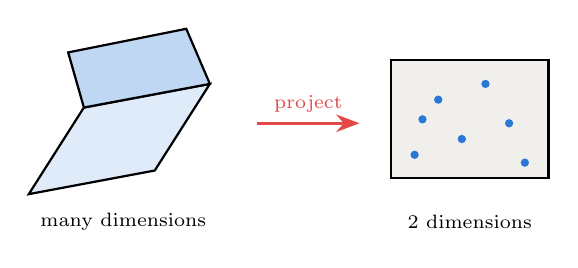
\begin{tikzpicture}[font=\scriptsize]
        % a 3D-ish object and its shadow
        \draw[thick,fill=bluemid!15] (0,0) -- (1.6,0.3) -- (2.3,1.4) -- (0.7,1.1) -- cycle;
        \draw[thick,fill=bluemid!30] (0.7,1.1) -- (2.3,1.4) -- (2.0,2.1) -- (0.5,1.8) -- cycle;
        \node at (1.2,-0.35) {many dimensions};
        \draw[-{Stealth},very thick,accentred] (2.9,0.9) -- node[above] {project} (4.2,0.9);
        \draw[thick,fill=softgrey] (4.6,0.2) rectangle (6.6,1.7);
        \foreach \x/\y in {4.9/0.5,5.2/1.2,5.5/0.7,5.8/1.4,6.1/0.9,6.3/0.4,5.0/0.95} \fill[bluemid] (\x,\y) circle (1.5pt);
        \node at (5.6,-0.35) {2 dimensions};
      \end{tikzpicture}\\[4pt]
      \footnotesize A good projection keeps the \alert{structure}: samples that are similar stay close.
    \end{column}
  \end{columns}
\end{frame}

\begin{frame}{PCA is a rotation}
  \begin{columns}[c]
    \begin{column}{0.52\linewidth}
      \centering
      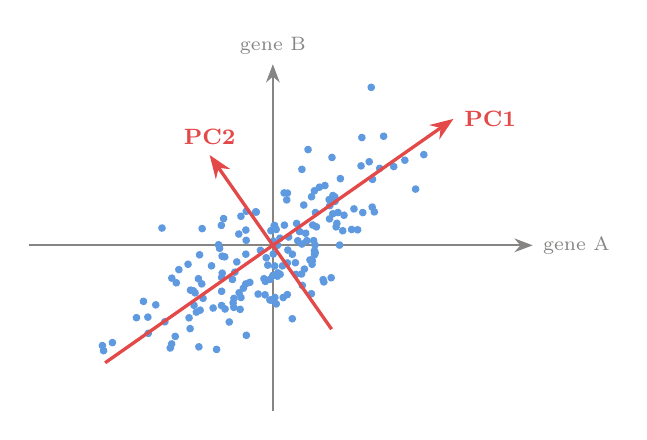
\begin{tikzpicture}[font=\scriptsize]
        \pgfmathsetseed{11}
        % original axes
        \draw[-{Stealth},thick,greyink!70] (-3.1,0) -- (3.3,0) node[right] {gene A};
        \draw[-{Stealth},thick,greyink!70] (0,-2.1) -- (0,2.3) node[above] {gene B};
        \begin{scope}[rotate=35]
          \foreach \i in {1,...,170} {
            \pgfmathsetmacro{\px}{(rnd+rnd+rnd-1.5)*2.0}
            \pgfmathsetmacro{\py}{(rnd+rnd+rnd-1.5)*0.7}
            \fill[bluemid!75] (\px,\py) circle (1.4pt);
          }
          \draw[-{Stealth},very thick,accentred] (-2.6,0) -- (2.8,0) node[right,font=\footnotesize\bfseries] {PC1};
          \draw[-{Stealth},very thick,accentred] (0,-1.3) -- (0,1.4) node[above,font=\footnotesize\bfseries] {PC2};
        \end{scope}
      \end{tikzpicture}
    \end{column}
    \begin{column}{0.46\linewidth}\small
      \begin{enumerate}\setlength\itemsep{4pt}
        \item \textbf{Centre} every gene (subtract its mean): the origin moves to the middle of the cloud.
        \item \textbf{Rotate} the axes until the first one points where the cloud is longest: that is \alert{PC1}. PC2 is perpendicular, and so on.
        \item Nothing is lost: a rotation keeps all the distances between samples.
      \end{enumerate}
      \vspace{0.2cm}
      \begin{block}{Dimensionality reduction}
        \footnotesize = keep only the first few PCs and forget the rest.
      \end{block}
    \end{column}
  \end{columns}
\end{frame}

\begin{frame}{How is it computed? The SVD}
  \centering
  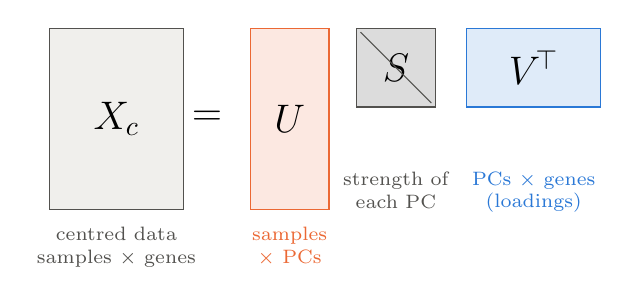
\begin{tikzpicture}[font=\scriptsize, every node/.style={align=center}]
    \node[draw=greyink,fill=softgrey,minimum width=1.7cm,minimum height=2.3cm] (X) at (0,0) {};
    \node at (0,0) {\Large $X_c$};
    \node at (1.15,0) {\Large $=$};
    \node[draw=orangeslot,fill=orangeslot!15,minimum width=1.0cm,minimum height=2.3cm] (U) at (2.2,0) {};
    \node at (2.2,0) {\Large $U$};
    \node[draw=greyink,fill=greyink!20,minimum width=1.0cm,minimum height=1.0cm] (S) at (3.55,0.65) {};
    \node at (3.55,0.65) {\Large $S$};
    \draw[greyink] (3.1,1.1) -- (4.0,0.2);
    \node[draw=bluemid,fill=bluemid!15,minimum width=1.7cm,minimum height=1.0cm] (V) at (5.3,0.65) {};
    \node at (5.3,0.65) {\Large $V^{\!\top}$};
    \node[text=greyink,below=0.1cm of X] {centred data\\ samples $\times$ genes};
    \node[text=orangeslot,below=0.1cm of U] {samples\\ $\times$ PCs};
    \node[text=greyink,below=0.7cm of S] {strength of\\ each PC};
    \node[text=bluemid,below=0.7cm of V] {PCs $\times$ genes\\ \alert{(loadings)}};
  \end{tikzpicture}
  \vspace{0.3cm}

  \begin{columns}[T]
    \begin{column}{0.5\linewidth}\small
      \begin{itemize}\setlength\itemsep{3pt}
        \item $V$ is a \alert{rotation}: its columns are the new axes (unit length, perpendicular): the weights of each gene in each PC.
        \item $S$: how much the data stretch along each axis.
      \end{itemize}
    \end{column}
    \begin{column}{0.46\linewidth}\small
      \begin{itemize}\setlength\itemsep{3pt}
        \item \textbf{Variance explained} by PC $k$: $\;s_k^2\big/\sum_j s_j^2$
        \item In Python: \code{np.linalg.svd(Xc)}; \code{scikit-learn}'s PCA does exactly this.
      \end{itemize}
    \end{column}
  \end{columns}
\end{frame}

\begin{frame}{Projection: scores and loadings}
  \centering
  \figfit[0.5]{p3_twogenes}
  \vspace{0.05cm}
  \begin{columns}[T]
    \begin{column}{0.5\linewidth}\small
      \begin{itemize}\setlength\itemsep{2pt}
        \item Monocytes, two genes (\gene{ISG15}, \gene{MX1}).
        \item The \alert{scores}, i.e.\ the coordinates of the samples on the new axes, are their \textbf{projection}: $T=X_c\,V=U\,S$
      \end{itemize}
    \end{column}
    \begin{column}{0.46\linewidth}\small
      \begin{itemize}\setlength\itemsep{2pt}
        \item Both loadings of PC1 are positive: PC1 $=$ ``overall interferon-gene level''.
        \item PC1 alone holds \alert{98\,\%} of the variance.
      \end{itemize}
    \end{column}
  \end{columns}
\end{frame}

\begin{frame}[fragile]{PCA in practice}
  \centering
  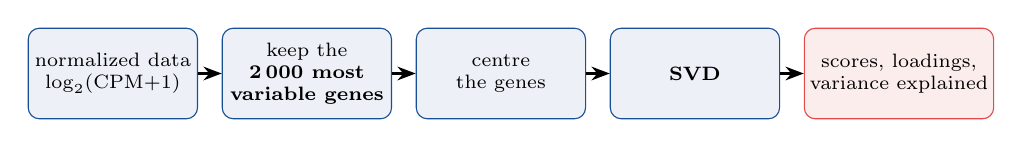
\begin{tikzpicture}[font=\scriptsize, every node/.style={align=center},
      stp/.style={draw=ucoblue,fill=ucoblue!8,rounded corners,minimum height=1.15cm,minimum width=2.15cm,inner sep=2pt}]
    \node[stp] (a) {normalized data\\ $\log_2$(CPM+1)};
    \node[stp,right=0.3cm of a] (b) {keep the\\ \textbf{2\,000 most}\\ \textbf{variable genes}};
    \node[stp,right=0.3cm of b] (c) {centre\\ the genes};
    \node[stp,right=0.3cm of c] (d) {\textbf{SVD}};
    \node[stp,right=0.3cm of d,fill=accentred!10,draw=accentred] (e) {scores, loadings,\\ variance explained};
    \foreach \x/\y in {a/b,b/c,c/d,d/e} \draw[-{Stealth},thick] (\x) -- (\y);
  \end{tikzpicture}
  \vspace{0.25cm}

\begin{lstlisting}
Mc = M - M.mean(axis=0)                          # 1) centre the genes
U, S, Vt = np.linalg.svd(Mc, full_matrices=False)   # 2) SVD
scores   = U * S                                 # 3) projection: samples on the PCs
loadings = Vt.T                                  #    weights of the genes
var_pct  = S**2 / (S**2).sum() * 100             #    % of variance of each PC
\end{lstlisting}
  \vspace{0.1cm}
  \small
  Then \alert{colour the samples} by metadata to find out what each PC means.
\end{frame}

\begin{frame}{PCA across fields}
  \centering
  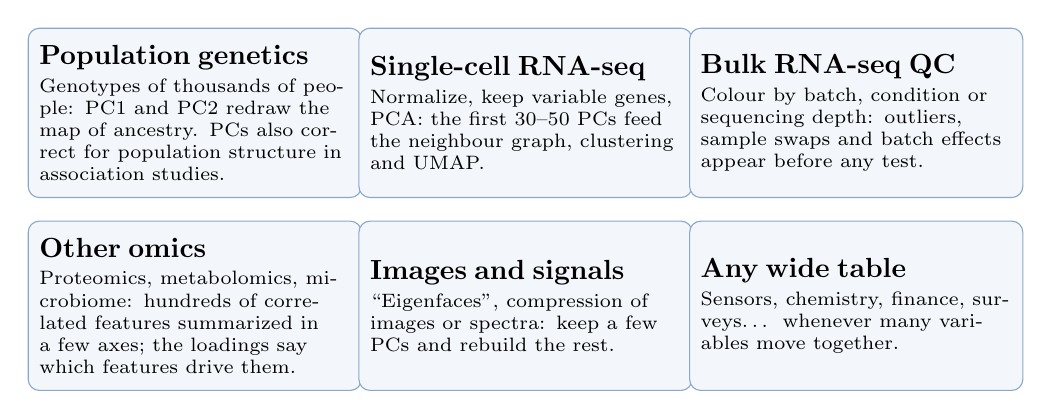
\begin{tikzpicture}[font=\scriptsize,
      card/.style={draw=ucoblue!50,rounded corners,fill=ucoblue!5,text width=3.95cm,inner sep=4pt,align=left,minimum height=2.15cm,anchor=north west}]
    \node[card] at (0,0)      {\textbf{\normalsize Population genetics}\\[2pt] Genotypes of thousands of people: PC1 and PC2 redraw the map of ancestry. PCs also correct for population structure in association studies.};
    \node[card] at (4.2,0)    {\textbf{\normalsize Single-cell RNA-seq}\\[2pt] Normalize, keep variable genes, PCA: the first 30--50 PCs feed the neighbour graph, clustering and UMAP.};
    \node[card] at (8.4,0)    {\textbf{\normalsize Bulk RNA-seq QC}\\[2pt] Colour by batch, condition or sequencing depth: outliers, sample swaps and batch effects appear before any test.};
    \node[card] at (0,-2.45)  {\textbf{\normalsize Other omics}\\[2pt] Proteomics, metabolomics, microbiome: hundreds of correlated features summarized in a few axes; the loadings say which features drive them.};
    \node[card] at (4.2,-2.45) {\textbf{\normalsize Images and signals}\\[2pt] ``Eigenfaces'', compression of images or spectra: keep a few PCs and rebuild the rest.};
    \node[card] at (8.4,-2.45) {\textbf{\normalsize Any wide table}\\[2pt] Sensors, chemistry, finance, surveys\ldots{} whenever many variables move together.};
  \end{tikzpicture}
  \vspace{0.1cm}

  \small In all of them PCA answers the same question: \alert{what are the main sources of variation in my data?}
\end{frame}

\begin{frame}{Reading PCA: colour first, interpret second}
  \begin{columns}[T]
    \begin{column}{0.52\linewidth}
      \begin{block}{How to find out what a PC means}
        \small
        \begin{enumerate}\setlength\itemsep{3pt}
          \item \textbf{Colour} the samples by every piece of metadata.
          \item Compute the \textbf{R$^2$} of each PC with each variable.
          \item Read the \textbf{loadings}: which genes define the axis?
        \end{enumerate}
      \end{block}
    \end{column}
    \begin{column}{0.44\linewidth}
      \begin{block}{What can go wrong}
        \footnotesize
        \begin{itemize}\setlength\itemsep{2pt}
          \item PCA finds the \alert{largest} variation, not the interesting one.
          \item Technical variables (depth, batch) can dominate: normalize first.
          \item A PC can mix several things (a cytokine axis and a sex axis in one PC).
          \item The sign of a PC is arbitrary. PCs are not clusters.
          \item It is exploratory: nothing is tested.
        \end{itemize}
      \end{block}
    \end{column}
  \end{columns}
\end{frame}

\begin{frame}{All samples: the cell type dominates}
  \centering
  \figfit[0.62]{p3_all_ct_donor}
  \begin{itemize}\small\setlength\itemsep{2pt}
    \item \textbf{PC1} (\numpcaone\,\%): monocytes vs lymphocytes. \textbf{PC2} (\numpcatwo\,\%): NK cells vs T cells.
    \item Inside every cell-type cluster the \alert{donors are mixed}: donor effects live on later PCs.
  \end{itemize}
\end{frame}

\begin{frame}{All samples: cytokines and control vs treated}
  \centering
  \figfit[0.62]{p3_all_cyt_trt}
  \begin{itemize}\small\setlength\itemsep{2pt}
    \item The PBS controls (black) sit \alert{inside} the cloud of treated samples. A few cytokines (IL-4) start to leave it.
    \item Cytokine effects are real but \alert{small compared with the cell-type differences}. Does that mean they do nothing?
  \end{itemize}
\end{frame}

\begin{frame}{Which PC captures what?}
  \centering
  \figfit[0.52]{p3_r2}
  \begin{itemize}\small\setlength\itemsep{2pt}
    \item PC1, PC2, PC4: \alert{cell type}. PC3, PC5, PC6, PC8: \alert{donor}.
    \item The first PC with cytokine signal is PC3 (R$^2$ 0.13): a low-variance PC. The first four PCs hold \numpcafirstfour\,\% of the variance.
    \item PC2 correlates with library size only because NK cells have smaller libraries: cell type in disguise.
  \end{itemize}
\end{frame}

\begin{frame}{What genes define a PC? The loadings}
  \centering
  \figfit[0.5]{p3_loadings}
  \begin{itemize}\small\setlength\itemsep{2pt}
    \item \textbf{PC1}: monocyte vs lymphocyte genes. \textbf{PC2}: NK genes (\gene{GNLY}, \gene{NCAM1}) vs naive-T genes (\gene{CCR7}, \gene{LEF1}).
    \item \textbf{PC3} mixes the \alert{interferon response} (\gene{IFIT1/2/3}, \gene{ISG15}) with \alert{Y-chromosome genes} (\gene{UTY}, \gene{USP9Y}): a cytokine axis and a sex axis in one PC.
  \end{itemize}
\end{frame}

\begin{frame}{Zoom in: monocytes only}
  \centering
  \figfit[0.62]{p3_mono_donor_cyt}
  \begin{itemize}\small\setlength\itemsep{2pt}
    \item \alert{Donors} form clear groups: baseline differences between people are large. Donor 2 stands apart (as in the paper).
    \item Cytokines do not separate yet. This is why Part 4 compares each cytokine with the PBS of the \alert{same donor}.
  \end{itemize}
\end{frame}

\begin{frame}{In the paper: donors differ before any treatment}
  \centering
  \includegraphics[width=0.95\linewidth,height=0.52\textheight,keepaspectratio]{paper_fig2_donors.png}\\[-1pt]
  {\tiny Oesinghaus \emph{et al.}\ 2025, Fig.\ 2a--g (CC BY-NC-ND 4.0)}
  \begin{itemize}\small\setlength\itemsep{2pt}
    \item A group of donors (D1, D3, D4, D10) has a \alert{high baseline interferon signature} in PBS (panels d, e): the paper's ``interferon group''; Donor 2 monocytes also sit apart (Fig.\ 2k), as in our PCA.
    \item These baseline differences are why we compare each cytokine with the PBS of the \alert{same donor}.
  \end{itemize}
\end{frame}

\begin{frame}{Monocytes: later PCs show the cytokines}
  \centering
  \figfit[0.64]{p3_mono_pc34}
  \begin{itemize}\small\setlength\itemsep{2pt}
    \item \textbf{IL-4} leaves the cloud towards low PC4, whose negative end holds IL-4 target genes (\gene{ALOX15}, \gene{WNT5B}, \gene{FN1}); \textbf{GM-CSF} goes towards high PC3.
    \item Each cytokine moves the samples in its \alert{own direction}, mixed with donor effects.
  \end{itemize}
\end{frame}

\begin{frame}{Your turn in the notebook (Part 3)}
  \small
  Cells that start with \code{\# CHANGE ME} contain parameters you can modify. Change them, re-run and see what happens:
  \vspace{0.2cm}

  \begin{tabular}{@{}>{\ttfamily}p{0.25\linewidth}>{\raggedright\arraybackslash}p{0.7\linewidth}@{}}
    \toprule
    \textrm{\textbf{Parameter}} & \textbf{Try\ldots}\\\midrule
    N\_HVG & $200$ and $10\,000$ genes: how robust is the picture?\\[2pt]
    CYTOKINES\_PANEL & six interferon-family cytokines: which ones cluster together?\\[2pt]
    PCA\_CELL\_TYPE & another cell type: does the cytokine effect look similar?\\[2pt]
    COLOR\_BY, PCS & a gene (\gene{UTY}, \gene{STAT1}, \gene{IL1B}), the library size, other PCs (PC3 vs PC4)\\
    \bottomrule
  \end{tabular}
\end{frame}

\begin{frame}{Part 3 in one slide}
  \begin{itemize}\setlength\itemsep{7pt}
    \item PCA is a \alert{rotation} of the data onto axes of decreasing variance, computed with the \alert{SVD}: \textbf{scores} = projection of the samples, \textbf{loadings} = weights of the genes.
    \item It is \alert{unsupervised}: colouring by metadata, R$^2$ and loadings tell what each PC means.
    \item \alert{Normalization} (Part 2) decides what PCA sees: without it, PC1 would be sequencing depth.
    \item The strongest variation is the \alert{cell type}; donor effects come next; cytokine effects are real but small and \alert{mixed with donor effects}.
    \item $\Rightarrow$ next: ask the question gene by gene, paired by donor.
  \end{itemize}
\end{frame}

% ════════════════════════════════════════════════════════════════════════════════════════
\section{Part 4: Differential expression}

\begin{frame}{Differential expression: the question and the pipeline}
  \centering
  \textit{For gene $g$: is the expression with the cytokine different from the expression with PBS, more than expected by chance?}\\[0.45cm]
  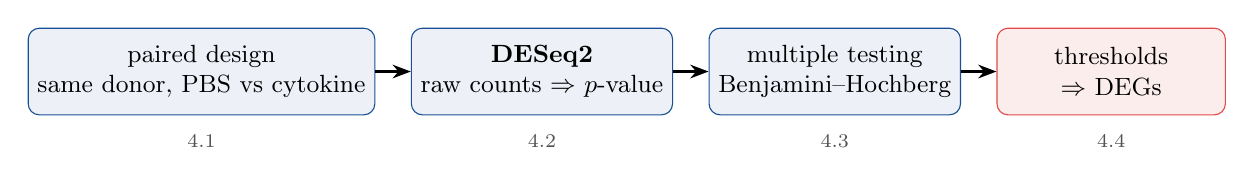
\begin{tikzpicture}[font=\small, every node/.style={align=center},
      box/.style={draw=ucoblue,fill=ucoblue!8,rounded corners,minimum height=1.1cm,minimum width=2.9cm}]
    \node[box] (a) {paired design\\ same donor, PBS vs cytokine};
    \node[box,right=0.45cm of a] (b) {\textbf{DESeq2}\\ raw counts $\Rightarrow$ $p$-value};
    \node[box,right=0.45cm of b] (c) {multiple testing\\ Benjamini--Hochberg};
    \node[box,right=0.45cm of c,fill=accentred!10,draw=accentred] (d) {thresholds\\ $\Rightarrow$ DEGs};
    \draw[-{Stealth},thick] (a) -- (b); \draw[-{Stealth},thick] (b) -- (c); \draw[-{Stealth},thick] (c) -- (d);
    \node[font=\scriptsize,text=greyink,below=0.12cm of a] {4.1};
    \node[font=\scriptsize,text=greyink,below=0.12cm of b] {4.2};
    \node[font=\scriptsize,text=greyink,below=0.12cm of c] {4.3};
    \node[font=\scriptsize,text=greyink,below=0.12cm of d] {4.4};
  \end{tikzpicture}
  \vspace{0.4cm}

  \begin{block}{Predict}
    In CD14 monocytes treated with \IFNg: more genes \textbf{up} or \textbf{down}? Tens, hundreds, thousands?
  \end{block}
\end{frame}

\begin{frame}{4.1 Paired design: every donor against itself}
  Each donor was measured with PBS \emph{and} with every cytokine; $y=\log_2(\text{CPM}+1)$:
  \[ d_{gi}=y^{\text{cytokine}}_{gi}-y^{\text{PBS}}_{gi}\qquad(g=\text{gene},\ i=1,\dots,12\ \text{donors}),\qquad \lfc_g=\bar d_g=\tfrac1{12}\textstyle\sum_i d_{gi} \]
  \begin{columns}[c]
    \begin{column}{0.55\linewidth}
      \figfit[0.52]{p4_paired}
    \end{column}
    \begin{column}{0.43\linewidth}\small
      \begin{itemize}\setlength\itemsep{3pt}
        \item Each line = one donor (red: higher with the cytokine).
        \item \gene{CXCL9}: every donor goes up, from different baselines. $\bar d=\numlfcobs$ ($\times\numfoldobs$).
        \item \gene{ACTB}: lines go both ways, no consistent change.
      \end{itemize}
    \end{column}
  \end{columns}
\end{frame}

\begin{frame}{4.1 The paired $t$-test, by hand}
  \begin{columns}[c]
    \begin{column}{0.48\linewidth}
      \[
        s_g=\sqrt{\tfrac1{n-1}\textstyle\sum_i(d_{gi}-\bar d_g)^2},\qquad
        t_g=\frac{\bar d_g}{s_g/\sqrt n}
      \]
      \[ p_g=2\,\Pr\bigl(T_{n-1}>|t_g|\bigr),\qquad n=12 \]
      \small
      \gene{CXCL9}, monocytes, \IFNg:
      \begin{itemize}\setlength\itemsep{1pt}
        \item $\bar d=\numlfcobs$, \quad $t=\numtobs$, \quad df $=11$
        \item $p=\numpobs$
      \end{itemize}
      Under H$_0$ (no effect) $t_g\sim t_{n-1}$. The $p$-value is the probability of a $|t|$ at least this large \emph{by chance}.
    \end{column}
    \begin{column}{0.5\linewidth}
      \figfit[0.6]{p4_tdist}
    \end{column}
  \end{columns}
\end{frame}

\begin{frame}{4.2 DESeq2: how does it work?}
  \centering
  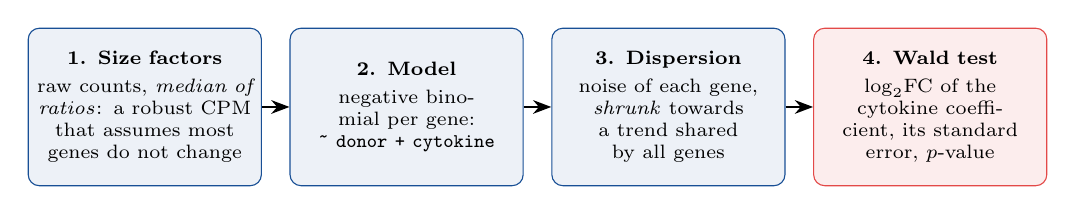
\begin{tikzpicture}[font=\scriptsize, every node/.style={align=center},
      stp/.style={draw=ucoblue,fill=ucoblue!8,rounded corners,minimum height=2.0cm,minimum width=2.95cm,inner sep=3pt,text width=2.75cm}]
    \node[stp] (a) {\textbf{1. Size factors}\\[2pt] raw counts, \emph{median of ratios}: a robust CPM that assumes most genes do not change};
    \node[stp,right=0.35cm of a] (b) {\textbf{2. Model}\\[2pt] negative binomial per gene:\\ \code{\textasciitilde\ donor + cytokine}};
    \node[stp,right=0.35cm of b] (c) {\textbf{3. Dispersion}\\[2pt] noise of each gene, \emph{shrunk} towards a trend shared by all genes};
    \node[stp,right=0.35cm of c,fill=accentred!10,draw=accentred] (d) {\textbf{4. Wald test}\\[2pt] $\log_2$FC of the cytokine coefficient, its standard error, $p$-value};
    \foreach \x/\y in {a/b,b/c,c/d} \draw[-{Stealth},thick] (\x) -- (\y);
  \end{tikzpicture}
  \vspace{0.25cm}

  \begin{columns}[T]
    \begin{column}{0.5\linewidth}\small
      \[ \log\mu_{gi}=\log s_i+\beta_{g,\text{donor}(i)}+\beta_{g,\text{cytokine}(i)} \]
      \begin{itemize}\setlength\itemsep{2pt}
        \item $s_i$: size factor of sample $i$. Counts are modelled, not log-CPM.
        \item \code{donor} gives each donor its own baseline: the \alert{paired design}.
      \end{itemize}
    \end{column}
    \begin{column}{0.46\linewidth}\small
      \begin{itemize}\setlength\itemsep{2pt}
        \item With only 12 donors, a gene's own noise is poorly estimated: sharing information across genes makes the test \alert{more stable}.
        \item In Python: \code{pydeseq2} (a port of the R package DESeq2, the field standard).
      \end{itemize}
    \end{column}
  \end{columns}
\end{frame}

\begin{frame}{4.2 DESeq2 under the hood}
  \centering
  \figfit[0.5]{p4_deseq_diag}
  \begin{itemize}\small\setlength\itemsep{2pt}
    \item \textbf{Size factors} (left) follow the library size, but are estimated from the genes that do not change, not from the total.
    \item \textbf{Dispersion} (right): the noise of each gene (grey) is \alert{pulled towards the trend} (red) to give the value used in the test (blue).
  \end{itemize}
\end{frame}

\begin{frame}{4.2 DESeq2 vs our log-CPM $t$-test}
  \centering
  \figfit[0.5]{p4_vs_ttest}
  \begin{itemize}\small\setlength\itemsep{2pt}
    \item Similar effect sizes ($r=\numreffect$). DEGs: DESeq2 \numndegdeseq, $t$-test \numndegt, \alert{both \numndegboth}.
    \item The median $\lfc$ is \nummediandeseq\ with DESeq2 but \nummediancpm\ with CPM: the \alert{composition effect} of Part 2, corrected by the median of ratios.
  \end{itemize}
\end{frame}

\begin{frame}{4.3 \numntested\ tests: raw $p$-values cannot be trusted}
  \centering
  \figfit[0.42]{p4_pvalues}
  \begin{itemize}\small\setlength\itemsep{2pt}
    \item \numntested\ genes tested at 5\,\% $\Rightarrow$ $\approx\numnexpectedfp$ false positives \emph{if nothing happens}.
    \item Null experiment (effects removed, signs of donors randomly flipped, $t$-test): \numnnullraw\ genes with $p<0.05$ and \alert{\numnnulladj} after correction.
    \item Real data: \numnrawsig\ genes with $p<0.05$: a spike near 0 on a flat floor.
  \end{itemize}
\end{frame}

\begin{frame}{Benjamini--Hochberg: controlling the false discovery rate}
  \begin{columns}[T]
    \begin{column}{0.52\linewidth}
      With $m$ tests and $p_{(1)}\le\dots\le p_{(m)}$:
      \[ p^{\mathrm{adj}}_{(i)}=\min_{k\ge i}\Bigl(\tfrac{m}{k}\,p_{(k)}\Bigr)\quad(\le1) \]
      \small
      \alert{FDR} $\le\alpha$: among the genes called significant at $\mathrm{padj}<0.05$, at most 5\,\% are expected to be false.\\[0.15cm]
      \scriptsize
      \begin{tabular}{lrrrr}\toprule
$i$ & $p_{(i)}$ & $p_{(i)}\,m/i$ & $p^{\mathrm{adj}}_{(i)}$ & sig.\\\midrule
1 & 0.001 & 0.010 & 0.010 & \checkmark\\
2 & 0.008 & 0.040 & 0.040 & \checkmark\\
3 & 0.012 & 0.040 & 0.040 & \checkmark\\
4 & 0.030 & 0.075 & 0.075 & \\
5 & 0.040 & 0.080 & 0.075 & \\
6 & 0.045 & 0.075 & 0.075 & \\
7 & 0.200 & 0.286 & 0.286 & \\
8 & 0.400 & 0.500 & 0.500 & \\
9 & 0.700 & 0.778 & 0.778 & \\
10 & 0.900 & 0.900 & 0.900 & \\
\bottomrule\end{tabular}

    \end{column}
    \begin{column}{0.44\linewidth}
      \figfit[0.62]{p4_bh}\\[-0.1cm]
      \scriptsize monocytes, \IFNg: sorted $p$-values and the line $\alpha k/m$. Everything up to $k^*=\numkstar$ is significant.
    \end{column}
  \end{columns}
\end{frame}

\begin{frame}{4.4 What do we call ``differentially expressed''?}
  \begin{columns}[c]
    \begin{column}{0.56\linewidth}
      \figfit[0.78]{p4_volcano}
    \end{column}
    \begin{column}{0.42\linewidth}\small
      \[
        \text{DEG}\;\Longleftrightarrow\;\mathrm{padj}<0.05\;\text{and}\;|\lfc|>0.5
      \]
      \begin{itemize}\setlength\itemsep{3pt}
        \item \textbf{Volcano}: effect size ($x$) against evidence ($y$). Significance $\neq$ importance: ask for both.
        \item Monocytes + \IFNg: \alert{\numnup\ up} and \alert{\numndown\ down} among \numntested\ tested genes.
        \item Labels: the strongest combination of effect and evidence. The classic IFN-$\gamma$ genes (\gene{CXCL9}, \gene{CXCL10}, \gene{IDO1}, \gene{GBP1}) are DEGs too.
      \end{itemize}
    \end{column}
  \end{columns}
\end{frame}

\begin{frame}{4.5 Comparing two cytokines}
  \centering
  \figfit[0.48]{p4_compare}\\[-2pt]
  \scriptsize
  \begin{tabular}{@{}lrrrrrr@{}}\toprule
cell type & IFN-gamma & IL-4 & both & only IFN-gamma & only IL-4 & IFN-gamma vs IL-4\\\midrule
CD14 monocyte & 2\,609 & 3\,748 & 1\,484 & 1\,125 & 2\,264 & 4\,755\\
CD4 T cell & 1\,024 & 1\,617 & 434 & 590 & 1\,183 & 2\,362\\
\bottomrule\end{tabular}

  \begin{itemize}\footnotesize\setlength\itemsep{1pt}
    \item Left: log$_2$FC of each cytokine vs PBS. Right: the direct comparison. Most DEGs are \alert{specific} to one cytokine.
  \end{itemize}
\end{frame}

\begin{frame}{In the paper: responses match known biology}
  \centering
  \includegraphics[width=0.7\linewidth,height=0.45\textheight,keepaspectratio]{paper_fig1de.png}\\[-1pt]
  {\tiny Oesinghaus \emph{et al.}\ 2025, Fig.\ 1d--e (CC BY-NC-ND 4.0)}
  \begin{itemize}\small\setlength\itemsep{2pt}
    \item Cytokine receptors and responses are cell-type specific (d); the induced genes (e) are the expected ones: IL-4 raises \gene{IL4R} and \gene{IL4I1} in B cells, IL-12 raises inflammatory and cytotoxicity genes in NK cells.
    \item The paper used \alert{edgeR} on pseudobulks with the design \code{\textasciitilde\ donor + cytokine}: the same idea as our \code{pydeseq2} analysis.
  \end{itemize}
\end{frame}

\begin{frame}{Your turn in the notebook (Part 4)}
  \small
  Cells that start with \code{\# CHANGE ME} contain parameters you can modify. Change them, re-run and see what happens:
  \vspace{0.2cm}

  \begin{tabular}{@{}>{\ttfamily}p{0.27\linewidth}>{\raggedright\arraybackslash}p{0.68\linewidth}@{}}
    \toprule
    \textrm{\textbf{Parameter}} & \textbf{Try\ldots}\\\midrule
    CYTOKINE, CELL\_TYPE & another cytokine (IL-4, TNF-alpha, IL-15\ldots) and cell type: how does the number of DEGs change?\\[2pt]
    EXAMPLE\_GENE & a gene you expect to respond (\gene{ALOX15} for IL-4): which gets the smallest $p$-value?\\[2pt]
    PADJ\_THRESH, LFC\_THRESH & $0.01$ and $1$: how many DEGs survive?\\[2pt]
    CYTOKINE\_A, CYTOKINE\_B & two interferons, or two members of the same family: which pair is the most similar?\\[2pt]
    CELL\_TYPES\_COMPARE & one or two cell types: where do the two cytokines differ most?\\
    \bottomrule
  \end{tabular}
\end{frame}

\begin{frame}{Caveats: a teaching model}
  \small
  \begin{tabular}{@{}>{\raggedright\arraybackslash}p{0.2\linewidth}>{\raggedright\arraybackslash}p{0.76\linewidth}@{}}
    \toprule
    \textbf{Design} & 12 donors: the unit of replication is the donor. \code{\textasciitilde\ donor + cytokine} removes baseline differences shared by both conditions, but donors with a high baseline interferon tone (the paper's ``interferon group'') respond differently.\\[3pt]
    \textbf{Tool} & DESeq2 is the standard, but not the only one: \texttt{edgeR} and \texttt{limma-voom} are alternatives. All need \alert{raw counts} and replicates.\\[3pt]
    \textbf{Pseudobulk} & Summing cells makes the donor the replicate. Testing single cells as if they were replicates inflates false positives.\\[3pt]
    \textbf{Filtering} & Remove untestable genes \emph{before} correcting for multiple testing.\\
    \bottomrule
  \end{tabular}
\end{frame}

\begin{frame}{Take-home messages}
  \small
  \begin{tabular}{@{}>{\raggedright\arraybackslash}p{0.27\linewidth}>{\raggedright\arraybackslash}p{0.69\linewidth}@{}}
    \toprule
    \textbf{Look first} & What is a count? How was the control built? How deep is each sample? Different cell types have very different library sizes.\\[2pt]
    \textbf{Normalize} & CPM for samples, $\log_2$ for genes, a filter for noise, z-scores only for heatmaps.\\[2pt]
    \textbf{PCA} & Shows what varies most (cell type, then donor); colour by metadata, check R$^2$ and loadings.\\[2pt]
    \textbf{Test} & DESeq2 on raw counts, paired by donor, with FDR correction and an effect-size threshold.\\[2pt]
    \textbf{Compare} & Two cytokines: shared and specific genes, and the direct contrast.\\[2pt]
    \textbf{Next step} & Turn DEG lists into biology with functional enrichment (pathways, transcription-factor targets).\\
    \bottomrule
  \end{tabular}
\end{frame}


% ════════════════════════════════════════════════════════════════════════════════════════
\section{Wrap-up}

\begin{frame}{The whole practical in one picture}
  \centering
  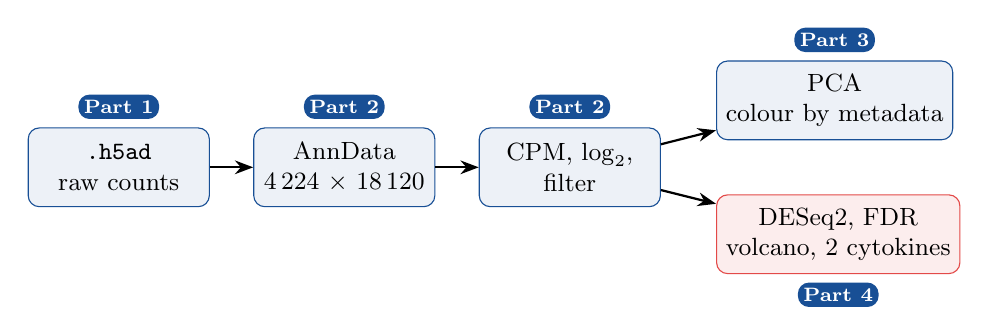
\begin{tikzpicture}[font=\small, every node/.style={align=center},
      box/.style={draw=ucoblue,fill=ucoblue!8,rounded corners,minimum height=1.0cm,minimum width=2.3cm},
      mod/.style={font=\scriptsize\bfseries,text=white,fill=ucoblue,rounded corners,inner sep=2pt}]
    \node[box] (h5) {\code{.h5ad}\\ raw counts};
    \node[box,right=0.55cm of h5] (an) {AnnData\\ \numnsamples\ $\times$ \numngenesraw};
    \node[box,right=0.55cm of an] (norm) {CPM, $\log_2$,\\ filter};
    \node[box,right=0.7cm of norm,yshift=0.85cm] (pca) {PCA\\ colour by metadata};
    \node[box,right=0.7cm of norm,yshift=-0.85cm,fill=accentred!10,draw=accentred] (de) {DESeq2, FDR\\ volcano, 2 cytokines};
    \draw[-{Stealth},thick] (h5) -- (an); \draw[-{Stealth},thick] (an) -- (norm);
    \draw[-{Stealth},thick] (norm) -- (pca); \draw[-{Stealth},thick] (norm) -- (de);
    \node[mod,above=0.1cm of h5] {Part 1}; \node[mod,above=0.1cm of an] {Part 2}; \node[mod,above=0.1cm of norm] {Part 2};
    \node[mod,above=0.1cm of pca] {Part 3}; \node[mod,below=0.1cm of de] {Part 4};
  \end{tikzpicture}
  \vspace{0.3cm}

  \begin{itemize}\small\setlength\itemsep{3pt}
    \item Look at the data before computing anything: what is a count, how was the control built, how deep is each sample?
    \item Normalize deliberately: samples, genes and heatmaps are three different problems.
    \item Let PCA show what varies; test what the question needs, paired by donor, corrected for multiple testing.
  \end{itemize}
\end{frame}

\begin{frame}{Quick quiz: 3 questions, 1 minute}
  \small
  Answer on the Google Form: \alert{[add the link or QR code of the form here]}
  \vspace{0.15cm}

  \begin{enumerate}\setlength\itemsep{6pt}
    \item Sample A has 5$\times$ more counts of \emph{every} gene than sample B, only because it was sequenced deeper. After CPM normalization, what do you expect for a gene that does not change?\\
      \textbf{a)} 5$\times$ higher in A \quad \textbf{b)} the same in A and B \quad \textbf{c)} 5$\times$ lower in A
    \item In the PCA of all the samples, what separates the samples most strongly (PC1)?\\
      \textbf{a)} the cytokine \quad \textbf{b)} the donor \quad \textbf{c)} the cell type \quad \textbf{d)} the library size
    \item Why do we use adjusted $p$-values (FDR) when we test $\sim$13\,000 genes?\\
      \textbf{a)} raw $p$-values are computed wrongly \quad \textbf{b)} to limit the false positives that appear by chance when many tests are done \quad \textbf{c)} to obtain more significant genes
  \end{enumerate}
\end{frame}

\appendix

\begin{frame}{Instructor only: answer key of the quiz}
  \small
  \begin{enumerate}\setlength\itemsep{6pt}
    \item \textbf{b)} CPM divides by the library size, so a gene that does not change has the same CPM in both samples (Part 2).
    \item \textbf{c)} The cell type: PC1 separates monocytes from lymphocytes and PC2 NK from T cells; cytokine effects are small by comparison (Part 3).
    \item \textbf{b)} At 5\,\% significance, $\sim$5\,\% of 13\,000 tests ($\approx$ 650 genes) are significant by chance if nothing happens; the Benjamini--Hochberg correction controls the false discovery rate (Part 4).
  \end{enumerate}
\end{frame}

\begin{frame}{References}
  \scriptsize
  \begin{itemize}\setlength\itemsep{3pt}
    \item Oesinghaus L.\ \emph{et al.} (2025) A single-cell cytokine dictionary of human peripheral blood. \emph{bioRxiv}. \texttt{doi:10.64898/2025.12.12.693897}
    \item Virshup I.\ \emph{et al.} (2024) anndata: Access and store annotated data matrices. \emph{J.\ Open Source Softw.} 9(101):4371.
    \item Heumos L.\ \emph{et al.} (2023) Best practices for single-cell analysis across modalities. \emph{Nat.\ Rev.\ Genet.} 24:550--572.
    \item Tzec-Interi\'an J.A., Gonz\'alez-Padilla D., G\'ongora-Castillo E.B. (2025) Bioinformatics perspectives on transcriptomics: a comprehensive review of bulk and single-cell RNA sequencing analyses. \emph{Quant.\ Biol.} e78. \texttt{doi:10.1002/qub2.78}
    \item Squair J.W.\ \emph{et al.} (2021) Confronting false discoveries in single-cell differential expression. \emph{Nat.\ Commun.} 12:5692.
    \item Benjamini Y., Hochberg Y. (1995) Controlling the false discovery rate. \emph{J.\ R.\ Stat.\ Soc.\ B} 57:289--300.
    \item Robinson M.D., McCarthy D.J., Smyth G.K. (2010) edgeR. \emph{Bioinformatics} 26:139--140.
    \item Muzellec B.\ \emph{et al.} (2023) PyDESeq2: a python package for bulk RNA-seq differential expression analysis. \emph{Bioinformatics} 39:btad547.
    \item Love M.I., Huber W., Anders S. (2014) Moderated estimation of fold change and dispersion for RNA-seq data with DESeq2. \emph{Genome Biol.} 15:550.
    \item Ritchie M.E.\ \emph{et al.} (2015) limma powers differential expression analyses for RNA-sequencing and microarray studies. \emph{Nucleic Acids Res.} 43:e47.
    \item Pedregosa F.\ \emph{et al.} (2011) Scikit-learn: machine learning in Python. \emph{J.\ Mach.\ Learn.\ Res.} 12:2825--2830.
  \end{itemize}
\end{frame}

\end{document}
